\documentclass{scrartcl}

\usepackage[utf8]{inputenc}
\usepackage[T1]{fontenc}
\usepackage{lmodern}
\usepackage{babel}
\usepackage{amsmath}
\usepackage{amsthm}
\usepackage{mathtools}
\usepackage[dvipsnames]{xcolor}
\usepackage{tikz}
\usepackage{pgfplots}
\usepackage{amssymb}
\usepackage{enumitem}
\usepackage{import}
\usepackage{subfigure}

\subimport{docs/libs/}{init}

\usetikzlibrary{patterns}
\usetikzlibrary{positioning}

\usepackage[
backend=biber,
% style=alphabetic,
sorting=none
]{biblatex}

\addbibresource{whitepaper.bib}

\title{Rule based Symbolic Reasoning}
\author{Matthias Lochbrunner}
\date{\today}

\theoremstyle{definition}
\newtheorem{exmp}{Example}[section]

\pgfplotsset{colormap/jet}

\tikzset{
    fromColorBar/.style={
        color of colormap={1000-#1*10},
        fill=.,
    },
}

\begin{document}
\maketitle
\begin{center}
	\textbf{Abstract}
\end{center}
\begin{abstract}
	The combination of a rule based beam search and deep learning is a promising approach to solve mathematical problems.
	One obstacle to overcome is the amount of possible branches in this search as the number of applicable rules and length of the calculation increases.
	This paper proposes to address this issue by constantly shrinking the beam size with a multi-head neuronal network:
	A policy head selects rules and positions in the current term.
	A value head evaluates the probability that this calculation could lead to the desired solution.
	Both heads help to reduce the beam size such that solving advanced mathematical problems becomes feasible.
\end{abstract}

\section{Motivation}

Since current approaches to solve mathematical problems use a complex but fixed set of rules, it takes manual effort to extend their capabilities \cite{wolfram}.
The generic approach described here might be able to incorporate additional rules without requiring manual work.
Moreover, it is not limited to mathematical problems as long as the domain can be described by a well-defined rule set.
The correctness of the result depends only on the correctness of the given rule set.

Gary Marcus proposes a hybrid, knowledge-driven, reasoning-based approach, centered around cognitive models,
that could provide the substrate for a richer, more robust AI than is currently possible. \cite{marcus2020decade}
This paper demonstrates one possible approach.

\section{Related work}

Lampe et. al. use state of the art sequence to sequence transformers (Vaswani et al. \cite{vaswani2017attention}) on equations formatted in the polish notation  \cite{Lample2020Deep}.
This approach views solving a mathematical problem as a translation problem.
% They don't use the concept of rules and tree structured data in the network.
Davis reviewed this work and come to the conclusion, that is astonishing that their transformer model outperforms contemporary computer algebra systems.
But he criticizes the limited vocabulary used in their generated data set \cite{davis2019use}.
In their latest paper they widened the scope of to five advanced mathematical problems and improved the many of the limitations discussed by the community \cite{charton2021learning}.
Inspired on that work Hahn et. al. also use a transformer based network for linear-time temporal logical formulas (LTL) \cite{hahn2021teaching}.
Similar to the result of the work by Lampe their method is capable to solve large formulas, but some results are semantically and syntactically wrong.

Lamb et al. presented a review on the relationship between GraphNeural Network (GNN) models and architectures and Neural-Symbolic Computing (NSC) \cite{lamb2020graph}.
They pointed out that this combination could provide trustful, explainable and robust AI systems.

Panju et at. build up a novel symbolic function learner to solve differential equations \cite{panju2020neurosymbolic}.
Their modeling approach is to iteratively feed the individual nodes of a syntax tree from the leaves to the root.
A very similar approach elaborated by Piepenbrock et al. \cite{piepenbrock2021learning}. 
% This method is able to approximate a symbolic function when the problem has no elementary symbolic solution.

A significant improvement is worked out by Rabe et al. They use an unsupervised proxy task to pre-train a sequence to sequence language model \cite{rabe2020mathematical}.
In their skip-tree training task the model is trained to predict a subtree in the syntax tree of an expression.
It is remarkable that they consider typed inference for variables and propositional logic to some extent.


\section{Method}

Given a problem, e.g. solve the equation $T_1\left(x\right)\equiv T_2\left(x\right)$ for $x$,
the beam search could try to apply various rules at different nodes in the syntax tree of the equation.
The policy head proposes the most promising combination of rules $R_j$ and positions $p_\ell$ in the current equation.
The value head evaluates the probability of success of the current calculation step.
The cumulative result of the value head can abort the solution path of the attempt, as it "seems" unlikely that the this attempt could succeed \cite{44806}.

\subsection{Rule Application}

A rule $R$ consists of one or multiple premises and one conclusion $B$.
In this paper we assume each rule to have only one premise $A$.
The outlook section discusses approaches rule of multiple premisses. 
Every rule is then of the shape $A \Longrightarrow B$ or $A \equiv B$, which is equivalent to $A \Longleftrightarrow B$ or just the combination of $A \Longrightarrow B$ and $B \Longrightarrow A$.
Without loss of correctness we just use the first shape $A \Longrightarrow B$ in this paper.
Let's name the term $T$ with the depth $d$ of the corresponding syntax tree representation.

\begin{figure}[!htbp]
	\centering
	\subfigure[Concrete symbols]  
{
\begin{tikzpicture}
    \node (=) at (0,0){$=$};
    \node (+) at (-1,-1){$+$};
    \node (-) at (1,-1){$-$};
    \node (a) at (-1.5, -2) {$a$};
    \node (b) at (-0.5, -2) {$b$};
    \node (c) at (0.5, -2) {$c$};
    \node (d) at (1.5, -2) {$d$};

    \draw[] (=) -- (+);
    \draw[] (=) -- (-);
    \draw[] (+) -- (a);
    \draw[] (+) -- (b);
    \draw[] (-) -- (c);
    \draw[] (-) -- (d);
\end{tikzpicture}
}
\subfigure[Index notation $t_p$]  
{
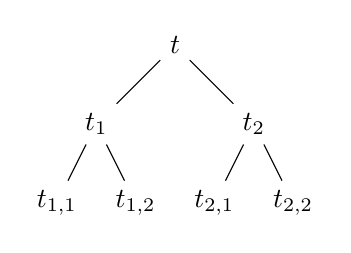
\begin{tikzpicture}
    \node (=) at (0,0){$t$};

    \node (+) at (-1,-1){$t_1$};
    \node (-) at (1,-1){$t_2$};
    \node (a) at (-1.5, -2) {$t_{1,1}$};
    \node (b) at (-0.5, -2) {$t_{1,2}$};
    \node (c) at (0.5, -2) {$t_{2,1}$};
    \node (d) at (1.5, -2) {$t_{2,2}$};

    \draw[] (=) -- (+);
    \draw[] (=) -- (-);
    \draw[] (+) -- (a);
    \draw[] (+) -- (b);
    \draw[] (-) -- (c);
    \draw[] (-) -- (d);
\end{tikzpicture}
}
\subfigure[Sub-terms $T_p$]  
{
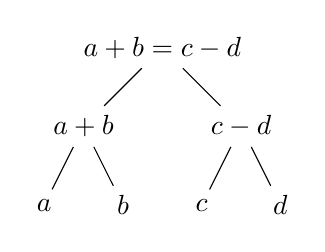
\begin{tikzpicture}
    \node (=) at (0,0){$a+b=c-d$};

    \node (+) at (-1,-1){$a+b$};
    \node (-) at (1,-1){$c-d$};
    \node (a) at (-1.5, -2) {$a$};
    \node (b) at (-0.5, -2) {$b$};
    \node (c) at (0.5, -2) {$c$};
    \node (d) at (1.5, -2) {$d$};

    \draw[] (=) -- (+);
    \draw[] (=) -- (-);
    \draw[] (+) -- (a);
    \draw[] (+) -- (b);
    \draw[] (-) -- (c);
    \draw[] (-) -- (d);
\end{tikzpicture}
}
\caption{
Example for of a syntax tree for the term $a+b=c-d$ with $s=2$.
To demonstrate the usage of position variable $p$ side by side the concrete symbols (a) and the here used notation $t_p$.
The sub term-terms are sub-figure (c)
}
	\label{fig:sxntax_tree}
\end{figure}

As the term $T$ can be represented by a tree we will name it's child terms $T_p$ with the position $p \in \big\{\left( n_1, n_2, \dots, n_d \right) | n_i \in \mathbb{N}, n_i \leq s \big\}$.
Hence the sub-terms of $T$ are $T_p$.
For instance $T_1$ is the sub-term at the first child node of the root node in that tree and $T_{1,1}$ is the first child term of $T_1$ and so on.
The root symbol of $T_p$ should be $t_p$.
Figure \ref{fig:sxntax_tree} demonstrates this notation by an example term.
Let $s$ be the maximal number of children per node in the syntax tree.

We try to match the premise term $A_j$ of rule $R_j$ at any position $p$ in term $T$.
Doing so results in a set of possible positions $p_\ell$ with the required substitution table ${M_{j,\ell}: S_{A_j} \to S_{T_{p_\ell}}}$,
where $S_{T_{p_\ell}}$ is the set of the sub-terms in term $T_{p_\ell}$ and $S_{A_j}$ the set of free symbols in the premise $A$.
Free symbols are symbols not defined elsewhere such as standard operators or the number $\pi$.
Then the application of that rule results in the new terms $T^{(j,\ell)}$ where each sub-term at $p_\ell$ gets replaced by the substituted conclusion ${B_j'^{(\ell)} \coloneqq M_{j,\ell}\left( B_j \right)}$.
Where $B_j'^{(\ell)}$ is $B_j$ with symbols mapped back by $M_{j,\ell}$. 

\begin{exmp}
To illustrate the above, let's look at the application of the derivative rule for polynomials.

Consider the derivative rule
\begin{align}
	\frac{\partial}{\partial {\color{red}x}} {\color{red}x}^{\color{blue}n} \Longrightarrow {\color{blue}n}\cdot {\color{red}x}^{{\color{blue}n}-1} 
\end{align}
with the premise $A\equiv \frac{\partial}{\partial {\color{red}x}} {\color{red}x}^{\color{blue}n}$ and the conclusion $B\equiv {\color{blue}n}\cdot {\color{red}x}^{{\color{blue}n}-1}$.
This rule can be applied to a sub-term of
\begin{align}
	a = \frac{\partial}{\partial {\color{red}z}} {\color{red}z}^{\color{blue}4} + b
	\label{example:problem}
\end{align}
at position $p=\left(2,1\right)$ where the derivative $\frac{\partial}{\partial {\color{red}z}} {\color{red}z}^{\color{blue}4}$ is located.
Using the symbol mapping $M\left({\color{red}x}\right) = \color{red}z$ and $M\left({\color{blue}n} \right) = {\color{blue}4}$ leads to the substituted conclusion
$B' = M(B) = M({\color{blue}n}\cdot {\color{red}x}^{{\color{blue}n}-1}) = {M(\color{blue}n})\cdot M({\color{red}x})^{M({\color{blue}n})-1} = {\color{blue}4}\cdot {\color{red}z}^{{\color{blue}4}-1}$.
Now you can replace the sub-term of equation (\ref{example:problem}) at position $p$ with with that $B'$ and obtain the resulting new term
\begin{align}
	a = {\color{blue}4}\cdot {\color{red}z}^{{\color{blue}4}-1} + b
\end{align}.

\end{exmp}

\subsection{Indexed Convolution for Tree Structured Data}

Lampe et. al. showed an approach where they unroll the term $T$ using the polish notation.
Then they apply contemporary NLP translation methods on that sequence where the resulting "translated sentence" is the next step in the calculation \cite{Lample2020Deep}.
The approach discussed here keeps the tree structure.
It turned out that a Tree-LSTM network performs poorly on that data \cite{tai2015improved}.

This paper will discuss the adoption of a network architectures using indexed convolution.
An attention based network with special positional encoding is discussed in the outlook. 

The indexed CNN operation performs a convolution of each node, with their it's neighbor nodes and itself.
Figure \ref{fig:index_tensor} demonstrates the operation by a simple example.

\begin{figure}[!htbp]
	\centering
	
    \tikzset{
        hatch distance/.store in=\hatchdistance,
        hatch distance=24pt,
        hatch thickness/.store in=\hatchthickness,
        hatch thickness=8pt
    }
\makeatletter
\pgfdeclarepatternformonly[\hatchdistance,\hatchthickness]{flexible hatch}
{\pgfqpoint{0pt}{0pt}}
{\pgfqpoint{\hatchdistance}{\hatchdistance}}
{\pgfpoint{\hatchdistance-1pt}{\hatchdistance-1pt}}%
{
    \pgfsetcolor{\tikz@pattern@color}
    \pgfsetlinewidth{\hatchthickness}
    \pgfpathmoveto{\pgfqpoint{0pt}{0pt}}
    \pgfpathlineto{\pgfqpoint{\hatchdistance}{\hatchdistance}}
    \pgfusepath{stroke}
}
\makeatother

\subfigure[Neighbors of the root.
$\scriptstyle \phi'_=={\color{red}w_1\phi_=}+{\color{blue}w_2\phi_+}+{\color{green!70!black}w_3\phi_-}+{\color{orange!80!black}w_4\phi_{\text{PAD}}}$]  
{
\tikzset{g_style/.style={black, draw=black!15, minimum size=0.5cm}}
\begin{tikzpicture}
    \node[g_style,fill=red!20,draw=black] (=) at (0,0){=};
    \node[g_style,fill=blue!20] (+) at (-1,-1){$+$};
    \node[g_style,fill=green!20] (-) at (1,-1){$-$};
    \node[g_style] (a) at (-1.5, -2) {$a$};
    \node[g_style] (b) at (-0.5, -2) {$b$};
    \node[g_style] (c) at (0.5, -2) {$c$};
    \node[g_style] (d) at (1.5, -2) {$d$};
    \node[g_style,fill=orange!20] at (1.5, 0) {\tiny PAD};

    \draw[draw=blue!70] (=) -- (+);
    \draw[draw=green!70] (=) -- (-);
    \draw[] (+) -- (a);
    \draw[] (+) -- (b);
    \draw[] (-) -- (c);
    \draw[] (-) -- (d);
\end{tikzpicture}
}
\subfigure[Neighbors of a left node $+$
$\scriptstyle \phi'_+={\color{red}w_1\phi_+}+{\color{blue}w_2\phi_a}+{\color{green!70!black}w_3\phi_b}+{\color{orange!80!black}w_4\phi_=}$]  
{
\tikzset{g_style/.style={black, draw=black!15, minimum size=0.5cm}}
\begin{tikzpicture}
    \node[g_style,fill=orange!20] (=) at (0,0){=};
    \node[g_style,fill=red!20,draw=black] (+) at (-1,-1){$+$};
    \node[g_style] (-) at (1,-1){$-$};
    \node[g_style,fill=blue!20] (a) at (-1.5, -2) {$a$};
    \node[g_style,fill=green!20] (b) at (-0.5, -2) {$b$};
    \node[g_style] (c) at (0.5, -2) {$c$};
    \node[g_style] (d) at (1.5, -2) {$d$};
    \node[g_style] at (1.5, 0) {\tiny PAD};

    \draw[draw=orange!70] (=) -- (+);
    \draw[] (=) -- (-);
    \draw[draw=blue!70] (+) -- (a);
    \draw[draw=green!70] (+) -- (b);
    \draw[] (-) -- (c);
    \draw[] (-) -- (d);
\end{tikzpicture}
}
\subfigure[Neighbors of a leaf $b$
$\scriptstyle \phi'_b={\color{red}w_1\phi_b}+{\color{blue}w_2\phi_{\text{PAD}}}+{\color{green!70!black}w_3\phi_{\text{PAD}}}+{\color{orange!80!black}w_4\phi_+}$]  
{
\tikzset{g_style/.style={black, draw=black!15, minimum size=0.5cm}}
\begin{tikzpicture}
    \node[g_style] (=) at (0,0){=};
    \node[g_style,fill=orange!20] (+) at (-1,-1){$+$};
    \node[g_style] (-) at (1,-1){$-$};
    \node[g_style] (a) at (-1.5, -2) {$a$};
    \node[g_style,fill=red!20,draw=black] (b) at (-0.5, -2) {$b$};
    \node[g_style] (c) at (0.5, -2) {$c$};
    \node[g_style] (d) at (1.5, -2) {$d$};
    {
        \node[preaction={fill=blue!20}, g_style, pattern=flexible hatch, pattern color=green!20] at (1.5, 0) {\tiny PAD};
    }

    \draw[] (=) -- (+);
    \draw[] (=) -- (-);
    \draw[] (+) -- (a);
    \draw[draw=orange!70] (+) -- (b);
    \draw[] (-) -- (c);
    \draw[] (-) -- (d);
\end{tikzpicture}
}
\caption{
    Example of indexed convolution operation on term $a+b=c+d$.
    Sub-figure (b) shows the computation of the next value $\phi' = C\left(\phi\right)$ for the node $a$ in that term.
    It is the weighted sum of the current values of itself, its children, and the parent.
    As the root in (a) has no parent node, we use the padding as a default node.
    The same is true for the child-nodes of a leaf in sub-figure (c).
    The colors red (self), blue (first child), green (second child), and orange (parent) indicated the neighbors of the focused node in each sub-plot.
}
	\label{fig:index_tensor}
\end{figure}

In order to increase the compute efficiency, each term is unrolled.
Let $t_p$ be the symbol at the root of sub-term $T_p$,
then the breadth-first unrolled term with $s=2$ is the vector $\left( t, t_1, t_2, t_{1,1},t_{1,2}, t_{2,1}, t_{2,2}, \cdots \right) \equiv  \left( t_{p_1}, t_{p_2}, t_{p_3},\cdots, t_{p_L} \right)$ of length $L$.
Hence in index notation $t_{p_\ell}$ where $1 \leq \ell \leq L$ is the index of symbol $t_p$ in the unrolled term.
An index map $g \in \mathbb{N}^{L\times \left(K\right)}$ carries the indices of the neighbors in a fixed order.
The kernel $K= s+2$ depends on the spread.
The index map of example in figure \ref{fig:index_tensor} would look like

\begin{align}
	g_{\ell,k} = 
	\begin{pmatrix}
		1 & 2 & 3 & 4 & 5 & 6 & 7 \\
		2 & 4 & 6 & 0 & 0 & 0 & 0 \\
		3 & 5 & 7 & 0 & 0 & 0 & 0 \\
		0 & 1 & 1 & 2 & 2 & 3 & 3 \\
	\end{pmatrix}^\top
\end{align}

where index $0$ points to the padding.


\begin{figure}[!htbp]
	\centering
	\def\ConvColor{rgb:yellow,5;red,2.5;white,5}
\def\ConvReluColor{rgb:yellow,5;red,5;white,5}

\begin{tikzpicture}
\tikzstyle{connection}=[ultra thick,every node/.style={sloped,allow upside down},draw=\edgecolor,opacity=0.7]

\pic[shift={(0,0,0)}] at (0,0,0) {RightBandedBox={name=ix,caption=input,%
        xlabel={{"t", "f"}},ylabel=L,zlabel=b,fill=\ConvColor,bandfill=\ConvColor,%
        height=8,width={2, 3},depth=8}};

\pic[shift={(0,3,0)}] at (0,0,0) {Box={name=i1,caption=indices,%
        xlabel={{"g"}},ylabel=L,zlabel=b,fill=\ConvColor,%
        height=8,width={2},depth=8}};

\pic[shift={(2,0,0)}] at (ix-east) {RightBandedBox={name=ic1,caption=iconv,%
        xlabel={{"e"}},ylabel=L,zlabel=b,fill=\ConvColor,bandfill=\ConvReluColor,%
        height=10,width={3},depth=10}};

\pic[shift={(4,0,0)}] at (ix-east) {RightBandedBox={name=ic2,caption=iconv,%
        xlabel={{"e"}},ylabel=L,zlabel=b,fill=\ConvColor,bandfill=\ConvReluColor,%
        height=10,width={3},depth=10}};

% heads

\pic[shift={(8,0,-4)}] at (ix-east) {RightBandedBox={name=icv,caption=iconv,%
xlabel={{"e"}},ylabel=L,zlabel=b,fill=\ConvColor,bandfill=\ConvReluColor,%
height=10,width={3},depth=10}};

\pic[shift={(10,0,-4)}] at (ix-east) {Box={name=ov,caption=value,%
xlabel={{"1"}},zlabel=b,ylabel=1,fill=\ConvColor,%
height=1,width={1},depth=10}};

\pic[shift={(8,0,4)}] at (ix-east) {RightBandedBox={name=icp,caption=iconv,%
        xlabel={{"e", "dummy"}},ylabel=L,zlabel=b,fill=\ConvColor,bandfill=\ConvReluColor,%
        height=10,width={3},depth=10}};

\pic[shift={(10,0,4)}] at (ix-east) {Box={name=op,caption=policy,%
        xlabel={{"r", "dummy"}},ylabel=L,zlabel=b,fill=\ConvColor,%
        height=10,width={8},depth=10}};


\path (ix-east) -- (ix-west) coordinate[pos=0.4] (after4) ;

\draw [connection] (ix-east) -- node {\midarrow} (ic1-west);
\draw [connection]  (ic1-east) -- node {\midarrow} (ic2-west);
\draw [connection]  (ic2-east) -- node {\midarrow} (icv-west);
\draw [connection]  (icv-east) -- node {\midarrow} (ov-west);
\draw [connection]  (ic2-east) -- node {\midarrow} (icp-west);
\draw [connection]  (icp-east) -- node {\midarrow} (op-west);

\draw [connection] (i1-east) -- ++ (2.5,0,0) -- node {\midarrow} (ic1-west);
\draw [connection] (i1-east) -- ++ (4.5,0,0) -- node {\midarrow} (ic2-west);
\draw [connection] (i1-east) -- ++ (5,0,0) -- ++ (3.5, 0, -4) -- node {\midarrow} (icv-west);
\draw [connection] (i1-east) -- ++ (5,0,0) -- ++ (3.5, 0, +4) -- node {\midarrow} (icp-west);

\end{tikzpicture}

	\caption{While $x\in \mathbb{R}^{L\times E}$ is the input tensor with $E$ encoded features per symbol $t_\ell$, the network needs the index tensor $g$ is an additional input.
		Each indexed convolution operations (iconv) reads from that index tensor.
		The policy head returns a matrix with the axis rule id $j$ and path id $\ell$. 
		The output of the value head is one scalar per sample in the mini-batch. 
	}
	\label{fig:iconv_network}
\end{figure}

Convolving over the input $x \in \mathbb{R}^{L\times I}$ with indexed convolution $C$ of with input channel $i \in \left[1,\cdots,I\right]$,
the kernel weights $w \in \mathbb{R}^{\left( s+2 \right)\times I \times J}$, output channel $j \in \left[1,\cdots,J\right]$ and bias $b \in \mathbb{R}^J$,
is defined as

\begin{align}
	C\left( x, g, w, b \right)_{\ell j} \coloneqq \sum_{ki}x_{g_{\ell k}i} w_{kij}+b_j
\end{align}

Figure \ref{fig:iconv_network} shows a overview of the multi-head network architecture, where the index tensor $g$ gets distributed to each indexed convolution layer.
These layers are used in the backbone and in the heads.
Due to the padding and stride of one the indexed convolution retains the shape of the input tensor, except of the configurable channel size.
This operation therefore is appropriate for stacking it to deep networks.
A deeper network leads to a larger receptive field and considers more distant symbols.

This is useful for the policy head, which assigns each sub-term a possibility estimation of the most promising rules to apply.

\begin{figure}[!htbp]
	\centering
	
% sample id: #19818
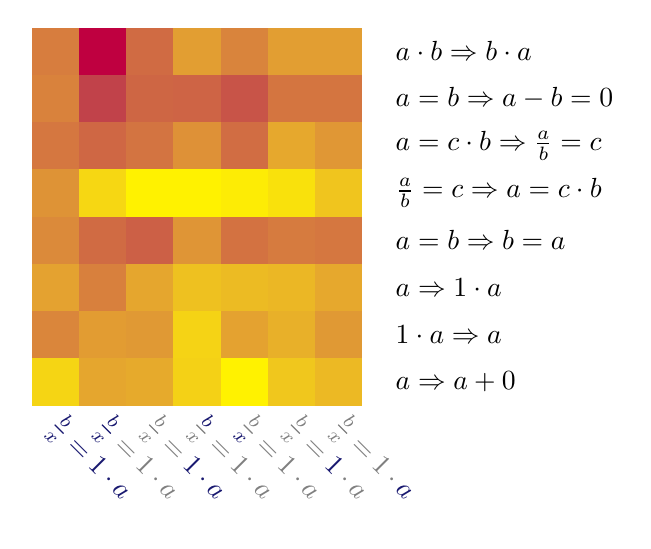
\begin{tikzpicture}[scale=0.6]
    \foreach \y [count=\p] in {
        {40,0,30,58,44,58,58},
        {43,6,27,26,17,36,36},
        {37,28,35,51,31,63,54},
        {52,87,100,100,97,92,78},
        {47,30,24,53,34,39,37},
        {60,42,62,76,73,71,63},
        {45,57,55,85,60,67,55},
        {86,62,64,84,100,79,72},
        } {
        \foreach \x [count=\r] in \y {
            \node[fill=yellow!\x!purple, minimum size=6mm, text=white] at (\r,-\p) {};
        }
    }
    \foreach \t [count=\p] in {
        $a\cdot b \Rightarrow b\cdot a $,
        $a=b \Rightarrow a-b=0 $,
        $a=c\cdot b \Rightarrow \frac{a}{b}=c $,
        $\frac{a}{b}=c \Rightarrow a=c\cdot b $,
        $a=b \Rightarrow b=a $,
        $a \Rightarrow 1\cdot a $,
        $1\cdot a \Rightarrow a $,
        $a \Rightarrow a+0 $
    } {
        \node[anchor=west] at (8, -\p) {\t};
    }
    \foreach \t [count=\r] in {
        $\textcolor{MidnightBlue}{\frac{b}{x}=1\cdot a}$,
        $\textcolor{Gray}{\textcolor{MidnightBlue}{\frac{b}{x}}=1\cdot a}$,
        $\textcolor{Gray}{\frac{b}{x}=\textcolor{MidnightBlue}{1\cdot a}}$,
        $\textcolor{Gray}{\frac{\textcolor{MidnightBlue}{b}}{x}=1\cdot a}$,
        $\textcolor{Gray}{\frac{b}{\textcolor{MidnightBlue}{x}}=1\cdot a}$,
        $\textcolor{Gray}{\frac{b}{x}=\textcolor{MidnightBlue}{1}\cdot a}$,
        $\textcolor{Gray}{\frac{b}{x}=1\cdot \textcolor{MidnightBlue}{a}}$
    } {
        \node[anchor=west, rotate=-45] at (\r - 0.2, -8.7) {\t};
    }
    \end{tikzpicture}
    
	\caption{Policy Network output: Each row is a possible rule $R_j$. Each column a sub-term $T_{p_\ell}$ of the initial term $T$ (highlighted in blue font).
	Rules which are not applicable to any $T_{p_\ell}$ are not shown here.
	}
	\label{fig:network_output}
\end{figure}

Figure \ref{fig:network_output} demonstrates the output of the policy head applied on the term $\frac{b}{x}=1\cdot a$.
% Find better example
This heat-map shows that dividing the equation by $a$ is more promising than blowing it up with the rules in in the in the at the bottom of the map.
The value head estimates the probability that the input term can lead to a solution.

\subsection{Three-T-Loop}

The training set consists of problems generated with computer algebra system Sympy \cite{10.7717/peerj-cs.103}.
A training sample is of a rule like shape $T^{(\text I)} \Longrightarrow T^{(\text T)}$ where $T^{(\text I)}$ is the initial problem term and $T^{(\text T)}$ the solution or target term.
The goal is to find the shortest chain of rule applications from the initial term to the target term:

\begin{align}
	T^{(\text I)} \Longrightarrow T^{(j_1)} \Longrightarrow T^{(j_1j_2)} \Longrightarrow \cdots \Longrightarrow T^{(\text T)}
	\label{eq:calculation_chain}
\end{align}

To obtain trainable data from the given problem set, we use an initial beam search without the assistance of a network.
A few simple problems can already be solved by this and learnable data can be extracted from these solution paths.
% Let's call this procedure \textit{three-T-loop} which consists of these three steps:
In order to solve more complex problems we choose an iterative approach.
The data loop consists of three steps:

% how is the network output used

\begin{enumerate}[label=(\roman*)]
	\item \textbf{Try} to solve some of the training problems.
	\item \textbf{Trace} the calculation steps of the solved problems and create training data out of them. 
	\item \textbf{Train} the model with the trainings data from the previous step.
\end{enumerate}
In each iteration of this \textit{three-T-loop}, the number of trainable data increases.
As the network's performance increases, it can solve more and more problems.
The trained network also reduces the number of misleading rule applications.
The value head helps to decide whether the calculation path seems promising to achieve a suitable result.
If the accumulated values are below a threshold the current path gets aborted to save resources (see Figure \ref{fig:beam_search} on page \pageref{fig:beam_search}). 

In order to get the model not doing the same mistake over and over again, it is important to train it with samples of paths which did not lead to a solution. 
These negative samples are present in the training set for value and policy head.


This loop can be extended by a forth step discussed in the outlook section, which allows to incorporate useful sub chains of formula (\ref{eq:calculation_chain}) into the rule set.

\begin{figure}[!htbp]
	\centering
	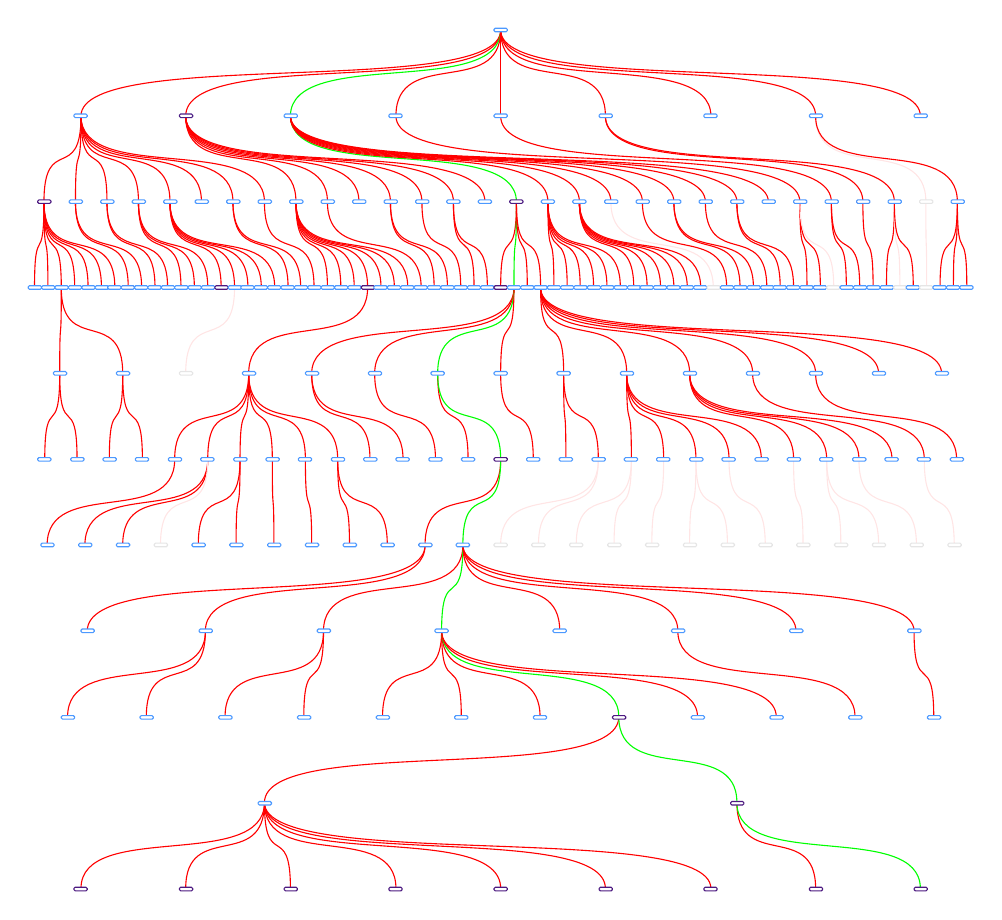
\begin{tikzpicture}[every node/.style={rectangle,fill=white,rounded corners=0.451}]
	\tikzset{xcolor/.code args={#1=#2}{
		\definecolor{mytemp}{rgb}{#2}
		\tikzset{draw=mytemp}
		}
	}
	\fontsize{0.5634}{0.6761}\selectfont
	\draw[draw=red] (-5.33,4.36) .. controls (-5.33,5.24) and (0.00,4.58) .. (0.00,5.45);
	\draw[draw=red] (-5.80,3.27) .. controls (-5.80,4.15) and (-5.33,3.49) .. (-5.33,4.36);
	\draw[draw=red] (-5.92,2.18) .. controls (-5.92,3.05) and (-5.80,2.40) .. (-5.80,3.27);
	\draw[draw=red] (-5.75,2.18) .. controls (-5.75,3.05) and (-5.80,2.40) .. (-5.80,3.27);
	\draw[draw=red] (-5.58,2.18) .. controls (-5.58,3.05) and (-5.80,2.40) .. (-5.80,3.27);
	\draw[draw=red] (-5.60,1.09) .. controls (-5.60,1.96) and (-5.58,1.31) .. (-5.58,2.18);
	\draw[draw=red] (-5.79,-8.88e-16) .. controls (-5.79,0.873) and (-5.60,0.218) .. (-5.60,1.09);
	\draw[draw=red] (-5.38,-8.88e-16) .. controls (-5.38,0.873) and (-5.60,0.218) .. (-5.60,1.09);
	\draw[draw=red] (-4.80,1.09) .. controls (-4.80,1.96) and (-5.58,1.31) .. (-5.58,2.18);
	\draw[draw=red] (-4.97,-8.88e-16) .. controls (-4.97,0.873) and (-4.80,0.218) .. (-4.80,1.09);
	\draw[draw=red] (-4.55,-8.88e-16) .. controls (-4.55,0.873) and (-4.80,0.218) .. (-4.80,1.09);
	\draw[draw=red] (-5.41,2.18) .. controls (-5.41,3.05) and (-5.80,2.40) .. (-5.80,3.27);
	\draw[draw=red] (-5.24,2.18) .. controls (-5.24,3.05) and (-5.80,2.40) .. (-5.80,3.27);
	\draw[draw=red] (-5.07,2.18) .. controls (-5.07,3.05) and (-5.80,2.40) .. (-5.80,3.27);
	\draw[draw=red] (-4.90,2.18) .. controls (-4.90,3.05) and (-5.80,2.40) .. (-5.80,3.27);
	\draw[draw=red] (-5.40,3.27) .. controls (-5.40,4.15) and (-5.33,3.49) .. (-5.33,4.36);
	\draw[draw=red] (-4.73,2.18) .. controls (-4.73,3.05) and (-5.40,2.40) .. (-5.40,3.27);
	\draw[draw=red] (-4.56,2.18) .. controls (-4.56,3.05) and (-5.40,2.40) .. (-5.40,3.27);
	\draw[draw=red] (-5.00,3.27) .. controls (-5.00,4.15) and (-5.33,3.49) .. (-5.33,4.36);
	\draw[draw=red] (-4.39,2.18) .. controls (-4.39,3.05) and (-5.00,2.40) .. (-5.00,3.27);
	\draw[draw=red] (-4.23,2.18) .. controls (-4.23,3.05) and (-5.00,2.40) .. (-5.00,3.27);
	\draw[draw=red] (-4.60,3.27) .. controls (-4.60,4.15) and (-5.33,3.49) .. (-5.33,4.36);
	\draw[draw=red] (-4.06,2.18) .. controls (-4.06,3.05) and (-4.60,2.40) .. (-4.60,3.27);
	\draw[draw=red] (-3.89,2.18) .. controls (-3.89,3.05) and (-4.60,2.40) .. (-4.60,3.27);
	\draw[draw=red] (-3.72,2.18) .. controls (-3.72,3.05) and (-4.60,2.40) .. (-4.60,3.27);
	\draw[draw=red] (-4.20,3.27) .. controls (-4.20,4.15) and (-5.33,3.49) .. (-5.33,4.36);
	\draw[draw=red] (-3.55,2.18) .. controls (-3.55,3.05) and (-4.20,2.40) .. (-4.20,3.27);
	\draw[draw=red] (-3.38,2.18) .. controls (-3.38,3.05) and (-4.20,2.40) .. (-4.20,3.27);
	\draw[draw=red!10] (-4.00,1.09) .. controls (-4.00,1.96) and (-3.38,1.31) .. (-3.38,2.18);
	\draw[draw=red] (-3.21,2.18) .. controls (-3.21,3.05) and (-4.20,2.40) .. (-4.20,3.27);
	\draw[draw=red] (-3.04,2.18) .. controls (-3.04,3.05) and (-4.20,2.40) .. (-4.20,3.27);
	\draw[draw=red] (-2.87,2.18) .. controls (-2.87,3.05) and (-4.20,2.40) .. (-4.20,3.27);
	\draw[draw=red] (-3.80,3.27) .. controls (-3.80,4.15) and (-5.33,3.49) .. (-5.33,4.36);
	\draw[draw=red] (-3.40,3.27) .. controls (-3.40,4.15) and (-5.33,3.49) .. (-5.33,4.36);
	\draw[draw=red] (-2.70,2.18) .. controls (-2.70,3.05) and (-3.40,2.40) .. (-3.40,3.27);
	\draw[draw=red] (-2.54,2.18) .. controls (-2.54,3.05) and (-3.40,2.40) .. (-3.40,3.27);
	\draw[draw=red] (-3.00,3.27) .. controls (-3.00,4.15) and (-5.33,3.49) .. (-5.33,4.36);
	\draw[draw=red] (-2.37,2.18) .. controls (-2.37,3.05) and (-3.00,2.40) .. (-3.00,3.27);
	\draw[draw=red] (-4.00,4.36) .. controls (-4.00,5.24) and (0.00,4.58) .. (0.00,5.45);
	\draw[draw=red] (-2.60,3.27) .. controls (-2.60,4.15) and (-4.00,3.49) .. (-4.00,4.36);
	\draw[draw=red] (-2.20,2.18) .. controls (-2.20,3.05) and (-2.60,2.40) .. (-2.60,3.27);
	\draw[draw=red] (-2.03,2.18) .. controls (-2.03,3.05) and (-2.60,2.40) .. (-2.60,3.27);
	\draw[draw=red] (-1.86,2.18) .. controls (-1.86,3.05) and (-2.60,2.40) .. (-2.60,3.27);
	\draw[draw=red] (-1.69,2.18) .. controls (-1.69,3.05) and (-2.60,2.40) .. (-2.60,3.27);
	\draw[draw=red] (-3.20,1.09) .. controls (-3.20,1.96) and (-1.69,1.31) .. (-1.69,2.18);
	\draw[draw=red] (-4.14,-8.88e-16) .. controls (-4.14,0.873) and (-3.20,0.218) .. (-3.20,1.09);
	\draw[draw=red] (-5.76,-1.09) .. controls (-5.76,-0.218) and (-4.14,-0.873) .. (-4.14,-8.88e-16);
	\draw[draw=red] (-3.72,-8.88e-16) .. controls (-3.72,0.873) and (-3.20,0.218) .. (-3.20,1.09);
	\draw[draw=red] (-5.28,-1.09) .. controls (-5.28,-0.218) and (-3.72,-0.873) .. (-3.72,-8.88e-16);
	\draw[draw=red] (-4.80,-1.09) .. controls (-4.80,-0.218) and (-3.72,-0.873) .. (-3.72,-8.88e-16);
	\draw[draw=red!10] (-4.32,-1.09) .. controls (-4.32,-0.218) and (-3.72,-0.873) .. (-3.72,-8.88e-16);
	\draw[draw=red] (-3.31,-8.88e-16) .. controls (-3.31,0.873) and (-3.20,0.218) .. (-3.20,1.09);
	\draw[draw=red] (-3.84,-1.09) .. controls (-3.84,-0.218) and (-3.31,-0.873) .. (-3.31,-8.88e-16);
	\draw[draw=red] (-3.36,-1.09) .. controls (-3.36,-0.218) and (-3.31,-0.873) .. (-3.31,-8.88e-16);
	\draw[draw=red] (-2.90,-8.88e-16) .. controls (-2.90,0.873) and (-3.20,0.218) .. (-3.20,1.09);
	\draw[draw=red] (-2.88,-1.09) .. controls (-2.88,-0.218) and (-2.90,-0.873) .. (-2.90,-8.88e-16);
	\draw[draw=red] (-2.48,-8.88e-16) .. controls (-2.48,0.873) and (-3.20,0.218) .. (-3.20,1.09);
	\draw[draw=red] (-2.40,-1.09) .. controls (-2.40,-0.218) and (-2.48,-0.873) .. (-2.48,-8.88e-16);
	\draw[draw=red] (-2.07,-8.88e-16) .. controls (-2.07,0.873) and (-3.20,0.218) .. (-3.20,1.09);
	\draw[draw=red] (-1.92,-1.09) .. controls (-1.92,-0.218) and (-2.07,-0.873) .. (-2.07,-8.88e-16);
	\draw[draw=red] (-1.44,-1.09) .. controls (-1.44,-0.218) and (-2.07,-0.873) .. (-2.07,-8.88e-16);
	\draw[draw=red] (-1.52,2.18) .. controls (-1.52,3.05) and (-2.60,2.40) .. (-2.60,3.27);
	\draw[draw=red] (-1.35,2.18) .. controls (-1.35,3.05) and (-2.60,2.40) .. (-2.60,3.27);
	\draw[draw=red] (-1.18,2.18) .. controls (-1.18,3.05) and (-2.60,2.40) .. (-2.60,3.27);
	\draw[draw=red] (-2.20,3.27) .. controls (-2.20,4.15) and (-4.00,3.49) .. (-4.00,4.36);
	\draw[draw=red] (-1.01,2.18) .. controls (-1.01,3.05) and (-2.20,2.40) .. (-2.20,3.27);
	\draw[draw=red] (-1.80,3.27) .. controls (-1.80,4.15) and (-4.00,3.49) .. (-4.00,4.36);
	\draw[draw=red] (-1.40,3.27) .. controls (-1.40,4.15) and (-4.00,3.49) .. (-4.00,4.36);
	\draw[draw=red] (-0.845,2.18) .. controls (-0.845,3.05) and (-1.40,2.40) .. (-1.40,3.27);
	\draw[draw=red] (-0.676,2.18) .. controls (-0.676,3.05) and (-1.40,2.40) .. (-1.40,3.27);
	\draw[draw=red] (-1.00,3.27) .. controls (-1.00,4.15) and (-4.00,3.49) .. (-4.00,4.36);
	\draw[draw=red] (-0.507,2.18) .. controls (-0.507,3.05) and (-1.00,2.40) .. (-1.00,3.27);
	\draw[draw=red] (-0.600,3.27) .. controls (-0.600,4.15) and (-4.00,3.49) .. (-4.00,4.36);
	\draw[draw=red] (-0.338,2.18) .. controls (-0.338,3.05) and (-0.600,2.40) .. (-0.600,3.27);
	\draw[draw=red] (-0.169,2.18) .. controls (-0.169,3.05) and (-0.600,2.40) .. (-0.600,3.27);
	\draw[draw=red] (-0.200,3.27) .. controls (-0.200,4.15) and (-4.00,3.49) .. (-4.00,4.36);
	\draw[draw=green] (-2.67,4.36) .. controls (-2.67,5.24) and (0.00,4.58) .. (0.00,5.45);
	\draw[draw=green] (0.200,3.27) .. controls (0.200,4.15) and (-2.67,3.49) .. (-2.67,4.36);
	\draw[draw=red] (0.00,2.18) .. controls (0.00,3.05) and (0.200,2.40) .. (0.200,3.27);
	\draw[draw=green] (0.169,2.18) .. controls (0.169,3.05) and (0.200,2.40) .. (0.200,3.27);
	\draw[draw=red] (-2.40,1.09) .. controls (-2.40,1.96) and (0.169,1.31) .. (0.169,2.18);
	\draw[draw=red] (-1.66,-8.88e-16) .. controls (-1.66,0.873) and (-2.40,0.218) .. (-2.40,1.09);
	\draw[draw=red] (-1.24,-8.88e-16) .. controls (-1.24,0.873) and (-2.40,0.218) .. (-2.40,1.09);
	\draw[draw=red] (-1.60,1.09) .. controls (-1.60,1.96) and (0.169,1.31) .. (0.169,2.18);
	\draw[draw=red] (-0.828,-8.88e-16) .. controls (-0.828,0.873) and (-1.60,0.218) .. (-1.60,1.09);
	\draw[draw=green] (-0.800,1.09) .. controls (-0.800,1.96) and (0.169,1.31) .. (0.169,2.18);
	\draw[draw=red] (-0.414,-8.88e-16) .. controls (-0.414,0.873) and (-0.800,0.218) .. (-0.800,1.09);
	\draw[draw=green] (0.00,-8.88e-16) .. controls (0.00,0.873) and (-0.800,0.218) .. (-0.800,1.09);
	\draw[draw=red] (-0.960,-1.09) .. controls (-0.960,-0.218) and (0.00,-0.873) .. (0.00,-8.88e-16);
	\draw[draw=red] (-5.25,-2.18) .. controls (-5.25,-1.31) and (-0.960,-1.96) .. (-0.960,-1.09);
	\draw[draw=red] (-3.75,-2.18) .. controls (-3.75,-1.31) and (-0.960,-1.96) .. (-0.960,-1.09);
	\draw[draw=red] (-5.50,-3.27) .. controls (-5.50,-2.40) and (-3.75,-3.05) .. (-3.75,-2.18);
	\draw[draw=red] (-4.50,-3.27) .. controls (-4.50,-2.40) and (-3.75,-3.05) .. (-3.75,-2.18);
	\draw[draw=green] (-0.480,-1.09) .. controls (-0.480,-0.218) and (0.00,-0.873) .. (0.00,-8.88e-16);
	\draw[draw=red] (-2.25,-2.18) .. controls (-2.25,-1.31) and (-0.480,-1.96) .. (-0.480,-1.09);
	\draw[draw=red] (-3.50,-3.27) .. controls (-3.50,-2.40) and (-2.25,-3.05) .. (-2.25,-2.18);
	\draw[draw=red] (-2.50,-3.27) .. controls (-2.50,-2.40) and (-2.25,-3.05) .. (-2.25,-2.18);
	\draw[draw=green] (-0.750,-2.18) .. controls (-0.750,-1.31) and (-0.480,-1.96) .. (-0.480,-1.09);
	\draw[draw=red] (-1.50,-3.27) .. controls (-1.50,-2.40) and (-0.750,-3.05) .. (-0.750,-2.18);
	\draw[draw=red] (-0.500,-3.27) .. controls (-0.500,-2.40) and (-0.750,-3.05) .. (-0.750,-2.18);
	\draw[draw=red] (0.500,-3.27) .. controls (0.500,-2.40) and (-0.750,-3.05) .. (-0.750,-2.18);
	\draw[draw=green] (1.50,-3.27) .. controls (1.50,-2.40) and (-0.750,-3.05) .. (-0.750,-2.18);
	\draw[draw=red] (-3.00,-4.36) .. controls (-3.00,-3.49) and (1.50,-4.15) .. (1.50,-3.27);
	\draw[draw=red] (-5.33,-5.45) .. controls (-5.33,-4.58) and (-3.00,-5.24) .. (-3.00,-4.36);
	\draw[draw=red] (-4.00,-5.45) .. controls (-4.00,-4.58) and (-3.00,-5.24) .. (-3.00,-4.36);
	\draw[draw=red] (-2.67,-5.45) .. controls (-2.67,-4.58) and (-3.00,-5.24) .. (-3.00,-4.36);
	\draw[draw=red] (-1.33,-5.45) .. controls (-1.33,-4.58) and (-3.00,-5.24) .. (-3.00,-4.36);
	\draw[draw=red] (0.00,-5.45) .. controls (0.00,-4.58) and (-3.00,-5.24) .. (-3.00,-4.36);
	\draw[draw=red] (1.33,-5.45) .. controls (1.33,-4.58) and (-3.00,-5.24) .. (-3.00,-4.36);
	\draw[draw=red] (2.67,-5.45) .. controls (2.67,-4.58) and (-3.00,-5.24) .. (-3.00,-4.36);
	\draw[draw=green] (3.00,-4.36) .. controls (3.00,-3.49) and (1.50,-4.15) .. (1.50,-3.27);
	\draw[draw=red] (4.00,-5.45) .. controls (4.00,-4.58) and (3.00,-5.24) .. (3.00,-4.36);
	\draw[draw=green] (5.33,-5.45) .. controls (5.33,-4.58) and (3.00,-5.24) .. (3.00,-4.36);
	\draw[draw=red] (2.50,-3.27) .. controls (2.50,-2.40) and (-0.750,-3.05) .. (-0.750,-2.18);
	\draw[draw=red] (3.50,-3.27) .. controls (3.50,-2.40) and (-0.750,-3.05) .. (-0.750,-2.18);
	\draw[draw=red] (0.750,-2.18) .. controls (0.750,-1.31) and (-0.480,-1.96) .. (-0.480,-1.09);
	\draw[draw=red] (2.25,-2.18) .. controls (2.25,-1.31) and (-0.480,-1.96) .. (-0.480,-1.09);
	\draw[draw=red] (4.50,-3.27) .. controls (4.50,-2.40) and (2.25,-3.05) .. (2.25,-2.18);
	\draw[draw=red] (3.75,-2.18) .. controls (3.75,-1.31) and (-0.480,-1.96) .. (-0.480,-1.09);
	\draw[draw=red] (5.25,-2.18) .. controls (5.25,-1.31) and (-0.480,-1.96) .. (-0.480,-1.09);
	\draw[draw=red] (5.50,-3.27) .. controls (5.50,-2.40) and (5.25,-3.05) .. (5.25,-2.18);
	\draw[draw=red] (8.88e-16,1.09) .. controls (8.88e-16,1.96) and (0.169,1.31) .. (0.169,2.18);
	\draw[draw=red] (0.414,-8.88e-16) .. controls (0.414,0.873) and (8.88e-16,0.218) .. (8.88e-16,1.09);
	\draw[draw=red] (0.338,2.18) .. controls (0.338,3.05) and (0.200,2.40) .. (0.200,3.27);
	\draw[draw=red] (0.507,2.18) .. controls (0.507,3.05) and (0.200,2.40) .. (0.200,3.27);
	\draw[draw=red] (0.800,1.09) .. controls (0.800,1.96) and (0.507,1.31) .. (0.507,2.18);
	\draw[draw=red] (0.828,-8.88e-16) .. controls (0.828,0.873) and (0.800,0.218) .. (0.800,1.09);
	\draw[draw=red] (1.24,-8.88e-16) .. controls (1.24,0.873) and (0.800,0.218) .. (0.800,1.09);
	\draw[draw=red!10] (0.00,-1.09) .. controls (0.00,-0.218) and (1.24,-0.873) .. (1.24,-8.88e-16);
	\draw[draw=red!10] (0.480,-1.09) .. controls (0.480,-0.218) and (1.24,-0.873) .. (1.24,-8.88e-16);
	\draw[draw=red] (1.60,1.09) .. controls (1.60,1.96) and (0.507,1.31) .. (0.507,2.18);
	\draw[draw=red] (1.66,-8.88e-16) .. controls (1.66,0.873) and (1.60,0.218) .. (1.60,1.09);
	\draw[draw=red!10] (0.960,-1.09) .. controls (0.960,-0.218) and (1.66,-0.873) .. (1.66,-8.88e-16);
	\draw[draw=red!10] (1.44,-1.09) .. controls (1.44,-0.218) and (1.66,-0.873) .. (1.66,-8.88e-16);
	\draw[draw=red] (2.07,-8.88e-16) .. controls (2.07,0.873) and (1.60,0.218) .. (1.60,1.09);
	\draw[draw=red!10] (1.92,-1.09) .. controls (1.92,-0.218) and (2.07,-0.873) .. (2.07,-8.88e-16);
	\draw[draw=red] (2.48,-8.88e-16) .. controls (2.48,0.873) and (1.60,0.218) .. (1.60,1.09);
	\draw[draw=red!10] (2.40,-1.09) .. controls (2.40,-0.218) and (2.48,-0.873) .. (2.48,-8.88e-16);
	\draw[draw=red!10] (2.88,-1.09) .. controls (2.88,-0.218) and (2.48,-0.873) .. (2.48,-8.88e-16);
	\draw[draw=red] (2.90,-8.88e-16) .. controls (2.90,0.873) and (1.60,0.218) .. (1.60,1.09);
	\draw[draw=red!10] (3.36,-1.09) .. controls (3.36,-0.218) and (2.90,-0.873) .. (2.90,-8.88e-16);
	\draw[draw=red] (3.31,-8.88e-16) .. controls (3.31,0.873) and (1.60,0.218) .. (1.60,1.09);
	\draw[draw=red] (2.40,1.09) .. controls (2.40,1.96) and (0.507,1.31) .. (0.507,2.18);
	\draw[draw=red] (3.72,-8.88e-16) .. controls (3.72,0.873) and (2.40,0.218) .. (2.40,1.09);
	\draw[draw=red!10] (3.84,-1.09) .. controls (3.84,-0.218) and (3.72,-0.873) .. (3.72,-8.88e-16);
	\draw[draw=red] (4.14,-8.88e-16) .. controls (4.14,0.873) and (2.40,0.218) .. (2.40,1.09);
	\draw[draw=red!10] (4.32,-1.09) .. controls (4.32,-0.218) and (4.14,-0.873) .. (4.14,-8.88e-16);
	\draw[draw=red!10] (4.80,-1.09) .. controls (4.80,-0.218) and (4.14,-0.873) .. (4.14,-8.88e-16);
	\draw[draw=red] (4.55,-8.88e-16) .. controls (4.55,0.873) and (2.40,0.218) .. (2.40,1.09);
	\draw[draw=red!10] (5.28,-1.09) .. controls (5.28,-0.218) and (4.55,-0.873) .. (4.55,-8.88e-16);
	\draw[draw=red] (4.97,-8.88e-16) .. controls (4.97,0.873) and (2.40,0.218) .. (2.40,1.09);
	\draw[draw=red] (3.20,1.09) .. controls (3.20,1.96) and (0.507,1.31) .. (0.507,2.18);
	\draw[draw=red] (5.38,-8.88e-16) .. controls (5.38,0.873) and (3.20,0.218) .. (3.20,1.09);
	\draw[draw=red!10] (5.76,-1.09) .. controls (5.76,-0.218) and (5.38,-0.873) .. (5.38,-8.88e-16);
	\draw[draw=red] (4.00,1.09) .. controls (4.00,1.96) and (0.507,1.31) .. (0.507,2.18);
	\draw[draw=red] (5.79,-8.88e-16) .. controls (5.79,0.873) and (4.00,0.218) .. (4.00,1.09);
	\draw[draw=red] (4.80,1.09) .. controls (4.80,1.96) and (0.507,1.31) .. (0.507,2.18);
	\draw[draw=red] (5.60,1.09) .. controls (5.60,1.96) and (0.507,1.31) .. (0.507,2.18);
	\draw[draw=red] (0.600,3.27) .. controls (0.600,4.15) and (-2.67,3.49) .. (-2.67,4.36);
	\draw[draw=red] (0.676,2.18) .. controls (0.676,3.05) and (0.600,2.40) .. (0.600,3.27);
	\draw[draw=red] (0.845,2.18) .. controls (0.845,3.05) and (0.600,2.40) .. (0.600,3.27);
	\draw[draw=red] (1.01,2.18) .. controls (1.01,3.05) and (0.600,2.40) .. (0.600,3.27);
	\draw[draw=red] (1.18,2.18) .. controls (1.18,3.05) and (0.600,2.40) .. (0.600,3.27);
	\draw[draw=red] (1.35,2.18) .. controls (1.35,3.05) and (0.600,2.40) .. (0.600,3.27);
	\draw[draw=red] (1.52,2.18) .. controls (1.52,3.05) and (0.600,2.40) .. (0.600,3.27);
	\draw[draw=red] (1.00,3.27) .. controls (1.00,4.15) and (-2.67,3.49) .. (-2.67,4.36);
	\draw[draw=red] (1.69,2.18) .. controls (1.69,3.05) and (1.00,2.40) .. (1.00,3.27);
	\draw[draw=red] (1.86,2.18) .. controls (1.86,3.05) and (1.00,2.40) .. (1.00,3.27);
	\draw[draw=red] (2.03,2.18) .. controls (2.03,3.05) and (1.00,2.40) .. (1.00,3.27);
	\draw[draw=red] (2.20,2.18) .. controls (2.20,3.05) and (1.00,2.40) .. (1.00,3.27);
	\draw[draw=red] (2.37,2.18) .. controls (2.37,3.05) and (1.00,2.40) .. (1.00,3.27);
	\draw[draw=red] (2.54,2.18) .. controls (2.54,3.05) and (1.00,2.40) .. (1.00,3.27);
	\draw[draw=red] (1.40,3.27) .. controls (1.40,4.15) and (-2.67,3.49) .. (-2.67,4.36);
	\draw[draw=red!10] (2.70,2.18) .. controls (2.70,3.05) and (1.40,2.40) .. (1.40,3.27);
	\draw[draw=red] (1.80,3.27) .. controls (1.80,4.15) and (-2.67,3.49) .. (-2.67,4.36);
	\draw[draw=red] (2.87,2.18) .. controls (2.87,3.05) and (1.80,2.40) .. (1.80,3.27);
	\draw[draw=red] (2.20,3.27) .. controls (2.20,4.15) and (-2.67,3.49) .. (-2.67,4.36);
	\draw[draw=red] (3.04,2.18) .. controls (3.04,3.05) and (2.20,2.40) .. (2.20,3.27);
	\draw[draw=red] (3.21,2.18) .. controls (3.21,3.05) and (2.20,2.40) .. (2.20,3.27);
	\draw[draw=red] (2.60,3.27) .. controls (2.60,4.15) and (-2.67,3.49) .. (-2.67,4.36);
	\draw[draw=red] (3.38,2.18) .. controls (3.38,3.05) and (2.60,2.40) .. (2.60,3.27);
	\draw[draw=red] (3.00,3.27) .. controls (3.00,4.15) and (-2.67,3.49) .. (-2.67,4.36);
	\draw[draw=red] (3.55,2.18) .. controls (3.55,3.05) and (3.00,2.40) .. (3.00,3.27);
	\draw[draw=red] (3.72,2.18) .. controls (3.72,3.05) and (3.00,2.40) .. (3.00,3.27);
	\draw[draw=red] (3.40,3.27) .. controls (3.40,4.15) and (-2.67,3.49) .. (-2.67,4.36);
	\draw[draw=red] (-1.33,4.36) .. controls (-1.33,5.24) and (0.00,4.58) .. (0.00,5.45);
	\draw[draw=red] (3.80,3.27) .. controls (3.80,4.15) and (-1.33,3.49) .. (-1.33,4.36);
	\draw[draw=red] (3.89,2.18) .. controls (3.89,3.05) and (3.80,2.40) .. (3.80,3.27);
	\draw[draw=red] (4.06,2.18) .. controls (4.06,3.05) and (3.80,2.40) .. (3.80,3.27);
	\draw[draw=red!10] (4.23,2.18) .. controls (4.23,3.05) and (3.80,2.40) .. (3.80,3.27);
	\draw[draw=red] (0.00,4.36) .. controls (0.00,5.24) and (0.00,4.58) .. (0.00,5.45);
	\draw[draw=red] (4.20,3.27) .. controls (4.20,4.15) and (0.00,3.49) .. (0.00,4.36);
	\draw[draw=red] (4.39,2.18) .. controls (4.39,3.05) and (4.20,2.40) .. (4.20,3.27);
	\draw[draw=red] (4.56,2.18) .. controls (4.56,3.05) and (4.20,2.40) .. (4.20,3.27);
	\draw[draw=red] (1.33,4.36) .. controls (1.33,5.24) and (0.00,4.58) .. (0.00,5.45);
	\draw[draw=red] (4.60,3.27) .. controls (4.60,4.15) and (1.33,3.49) .. (1.33,4.36);
	\draw[draw=red] (4.73,2.18) .. controls (4.73,3.05) and (4.60,2.40) .. (4.60,3.27);
	\draw[draw=red] (5.00,3.27) .. controls (5.00,4.15) and (1.33,3.49) .. (1.33,4.36);
	\draw[draw=red] (4.90,2.18) .. controls (4.90,3.05) and (5.00,2.40) .. (5.00,3.27);
	\draw[draw=red!10] (5.07,2.18) .. controls (5.07,3.05) and (5.00,2.40) .. (5.00,3.27);
	\draw[draw=red] (5.24,2.18) .. controls (5.24,3.05) and (5.00,2.40) .. (5.00,3.27);
	\draw[draw=red] (2.67,4.36) .. controls (2.67,5.24) and (0.00,4.58) .. (0.00,5.45);
	\draw[draw=red] (4.00,4.36) .. controls (4.00,5.24) and (0.00,4.58) .. (0.00,5.45);
	\draw[draw=red!10] (5.40,3.27) .. controls (5.40,4.15) and (4.00,3.49) .. (4.00,4.36);
	\draw[draw=red!10] (5.41,2.18) .. controls (5.41,3.05) and (5.40,2.40) .. (5.40,3.27);
	\draw[draw=red] (5.80,3.27) .. controls (5.80,4.15) and (4.00,3.49) .. (4.00,4.36);
	\draw[draw=red] (5.58,2.18) .. controls (5.58,3.05) and (5.80,2.40) .. (5.80,3.27);
	\draw[draw=red] (5.75,2.18) .. controls (5.75,3.05) and (5.80,2.40) .. (5.80,3.27);
	\draw[draw=red] (5.92,2.18) .. controls (5.92,3.05) and (5.80,2.40) .. (5.80,3.27);
	\draw[draw=red] (5.33,4.36) .. controls (5.33,5.24) and (0.00,4.58) .. (0.00,5.45);
	\filldraw[fill=white, xcolor={a color={0.3, 0.6, 1}}, rounded corners=0.451] (-0.0845,5.43) rectangle ++ (0.169,0.0451);
	\filldraw[fill=white, xcolor={a color={0.3, 0.6, 1}}, rounded corners=0.451] (-5.42,4.34) rectangle ++ (0.169,0.0451);
	\filldraw[fill=white, xcolor={a color={0.3, 0.10000000022363711, 0.5000000002236371}}, rounded corners=0.451] (-5.88,3.25) rectangle ++ (0.169,0.0451);
	\filldraw[fill=white, xcolor={a color={0.3, 0.6, 1}}, rounded corners=0.451] (-6.00,2.16) rectangle ++ (0.169,0.0451);
	\filldraw[fill=white, xcolor={a color={0.3, 0.6, 1}}, rounded corners=0.451] (-5.83,2.16) rectangle ++ (0.169,0.0451);
	\filldraw[fill=white, xcolor={a color={0.3, 0.6, 1}}, rounded corners=0.451] (-5.66,2.16) rectangle ++ (0.169,0.0451);
	\filldraw[fill=white, xcolor={a color={0.3, 0.6, 1}}, rounded corners=0.451] (-5.68,1.07) rectangle ++ (0.169,0.0451);
	\filldraw[fill=white, xcolor={a color={0.3, 0.6, 1}}, rounded corners=0.451] (-5.88,-0.0225) rectangle ++ (0.169,0.0451);
	\filldraw[fill=white, xcolor={a color={0.3, 0.6, 1}}, rounded corners=0.451] (-5.46,-0.0225) rectangle ++ (0.169,0.0451);
	\filldraw[fill=white, xcolor={a color={0.3, 0.6, 1}}, rounded corners=0.451] (-4.88,1.07) rectangle ++ (0.169,0.0451);
	\filldraw[fill=white, xcolor={a color={0.3, 0.6, 1}}, rounded corners=0.451] (-5.05,-0.0225) rectangle ++ (0.169,0.0451);
	\filldraw[fill=white, xcolor={a color={0.3, 0.6, 1}}, rounded corners=0.451] (-4.64,-0.0225) rectangle ++ (0.169,0.0451);
	\filldraw[fill=white, xcolor={a color={0.3, 0.6, 1}}, rounded corners=0.451] (-5.49,2.16) rectangle ++ (0.169,0.0451);
	\filldraw[fill=white, xcolor={a color={0.3, 0.5999916851520538, 0.9999916851520538}}, rounded corners=0.451] (-5.32,2.16) rectangle ++ (0.169,0.0451);
	\filldraw[fill=white, xcolor={a color={0.3, 0.5999999701976776, 0.9999999701976776}}, rounded corners=0.451] (-5.15,2.16) rectangle ++ (0.169,0.0451);
	\filldraw[fill=white, xcolor={a color={0.3, 0.6, 1}}, rounded corners=0.451] (-4.99,2.16) rectangle ++ (0.169,0.0451);
	\filldraw[fill=white, xcolor={a color={0.3, 0.6, 1}}, rounded corners=0.451] (-5.48,3.25) rectangle ++ (0.169,0.0451);
	\filldraw[fill=white, xcolor={a color={0.3, 0.5743517637252807, 0.9743517637252808}}, rounded corners=0.451] (-4.82,2.16) rectangle ++ (0.169,0.0451);
	\filldraw[fill=white, xcolor={a color={0.3, 0.6, 1}}, rounded corners=0.451] (-4.65,2.16) rectangle ++ (0.169,0.0451);
	\filldraw[fill=white, xcolor={a color={0.3, 0.6, 1}}, rounded corners=0.451] (-5.08,3.25) rectangle ++ (0.169,0.0451);
	\filldraw[fill=white, xcolor={a color={0.3, 0.6, 1}}, rounded corners=0.451] (-4.48,2.16) rectangle ++ (0.169,0.0451);
	\filldraw[fill=white, xcolor={a color={0.3, 0.6, 1}}, rounded corners=0.451] (-4.31,2.16) rectangle ++ (0.169,0.0451);
	\filldraw[fill=white, xcolor={a color={0.3, 0.6, 1}}, rounded corners=0.451] (-4.68,3.25) rectangle ++ (0.169,0.0451);
	\filldraw[fill=white, xcolor={a color={0.3, 0.6, 1}}, rounded corners=0.451] (-4.14,2.16) rectangle ++ (0.169,0.0451);
	\filldraw[fill=white, xcolor={a color={0.3, 0.6, 1}}, rounded corners=0.451] (-3.97,2.16) rectangle ++ (0.169,0.0451);
	\filldraw[fill=white, xcolor={a color={0.3, 0.6, 1}}, rounded corners=0.451] (-3.80,2.16) rectangle ++ (0.169,0.0451);
	\filldraw[fill=white, xcolor={a color={0.3, 0.6, 1}}, rounded corners=0.451] (-4.28,3.25) rectangle ++ (0.169,0.0451);
	\filldraw[fill=white, xcolor={a color={0.3, 0.10000479798791276, 0.5000047979879128}}, rounded corners=0.451] (-3.63,2.16) rectangle ++ (0.169,0.0451);
	\filldraw[fill=white, xcolor={a color={0.3, 0.6, 1}}, rounded corners=0.451] (-3.46,2.16) rectangle ++ (0.169,0.0451);
	\filldraw[fill=white, xcolor={a color={0.9,0.9,0.9}}, rounded corners=0.451] (-4.08,1.07) rectangle ++ (0.169,0.0451);
	\filldraw[fill=white, xcolor={a color={0.3, 0.6, 1}}, rounded corners=0.451] (-3.30,2.16) rectangle ++ (0.169,0.0451);
	\filldraw[fill=white, xcolor={a color={0.3, 0.6, 1}}, rounded corners=0.451] (-3.13,2.16) rectangle ++ (0.169,0.0451);
	\filldraw[fill=white, xcolor={a color={0.3, 0.6, 1}}, rounded corners=0.451] (-2.96,2.16) rectangle ++ (0.169,0.0451);
	\filldraw[fill=white, xcolor={a color={0.3, 0.6, 1}}, rounded corners=0.451] (-3.88,3.25) rectangle ++ (0.169,0.0451);
	\filldraw[fill=white, xcolor={a color={0.3, 0.6, 1}}, rounded corners=0.451] (-3.48,3.25) rectangle ++ (0.169,0.0451);
	\filldraw[fill=white, xcolor={a color={0.3, 0.6, 1}}, rounded corners=0.451] (-2.79,2.16) rectangle ++ (0.169,0.0451);
	\filldraw[fill=white, xcolor={a color={0.3, 0.6, 1}}, rounded corners=0.451] (-2.62,2.16) rectangle ++ (0.169,0.0451);
	\filldraw[fill=white, xcolor={a color={0.3, 0.6, 1}}, rounded corners=0.451] (-3.08,3.25) rectangle ++ (0.169,0.0451);
	\filldraw[fill=white, xcolor={a color={0.3, 0.6, 1}}, rounded corners=0.451] (-2.45,2.16) rectangle ++ (0.169,0.0451);
	\filldraw[fill=white, xcolor={a color={0.3, 0.12492575719952584, 0.5249257571995258}}, rounded corners=0.451] (-4.08,4.34) rectangle ++ (0.169,0.0451);
	\filldraw[fill=white, xcolor={a color={0.3, 0.6, 1}}, rounded corners=0.451] (-2.68,3.25) rectangle ++ (0.169,0.0451);
	\filldraw[fill=white, xcolor={a color={0.3, 0.6, 1}}, rounded corners=0.451] (-2.28,2.16) rectangle ++ (0.169,0.0451);
	\filldraw[fill=white, xcolor={a color={0.3, 0.6, 1}}, rounded corners=0.451] (-2.11,2.16) rectangle ++ (0.169,0.0451);
	\filldraw[fill=white, xcolor={a color={0.3, 0.6, 1}}, rounded corners=0.451] (-1.94,2.16) rectangle ++ (0.169,0.0451);
	\filldraw[fill=white, xcolor={a color={0.3, 0.1017418924253434, 0.5017418924253434}}, rounded corners=0.451] (-1.77,2.16) rectangle ++ (0.169,0.0451);
	\filldraw[fill=white, xcolor={a color={0.3, 0.6, 1}}, rounded corners=0.451] (-3.28,1.07) rectangle ++ (0.169,0.0451);
	\filldraw[fill=white, xcolor={a color={0.3, 0.6, 1}}, rounded corners=0.451] (-4.22,-0.0225) rectangle ++ (0.169,0.0451);
	\filldraw[fill=white, xcolor={a color={0.3, 0.6, 1}}, rounded corners=0.451] (-5.84,-1.11) rectangle ++ (0.169,0.0451);
	\filldraw[fill=white, xcolor={a color={0.3, 0.6, 1}}, rounded corners=0.451] (-3.81,-0.0225) rectangle ++ (0.169,0.0451);
	\filldraw[fill=white, xcolor={a color={0.3, 0.6, 1}}, rounded corners=0.451] (-5.36,-1.11) rectangle ++ (0.169,0.0451);
	\filldraw[fill=white, xcolor={a color={0.3, 0.6, 1}}, rounded corners=0.451] (-4.88,-1.11) rectangle ++ (0.169,0.0451);
	\filldraw[fill=white, xcolor={a color={0.9,0.9,0.9}}, rounded corners=0.451] (-4.40,-1.11) rectangle ++ (0.169,0.0451);
	\filldraw[fill=white, xcolor={a color={0.3, 0.6, 1}}, rounded corners=0.451] (-3.39,-0.0225) rectangle ++ (0.169,0.0451);
	\filldraw[fill=white, xcolor={a color={0.3, 0.6, 1}}, rounded corners=0.451] (-3.92,-1.11) rectangle ++ (0.169,0.0451);
	\filldraw[fill=white, xcolor={a color={0.3, 0.6, 1}}, rounded corners=0.451] (-3.44,-1.11) rectangle ++ (0.169,0.0451);
	\filldraw[fill=white, xcolor={a color={0.3, 0.6, 1}}, rounded corners=0.451] (-2.98,-0.0225) rectangle ++ (0.169,0.0451);
	\filldraw[fill=white, xcolor={a color={0.3, 0.6, 1}}, rounded corners=0.451] (-2.96,-1.11) rectangle ++ (0.169,0.0451);
	\filldraw[fill=white, xcolor={a color={0.3, 0.6, 1}}, rounded corners=0.451] (-2.57,-0.0225) rectangle ++ (0.169,0.0451);
	\filldraw[fill=white, xcolor={a color={0.3, 0.6, 1}}, rounded corners=0.451] (-2.48,-1.11) rectangle ++ (0.169,0.0451);
	\filldraw[fill=white, xcolor={a color={0.3, 0.6, 1}}, rounded corners=0.451] (-2.15,-0.0225) rectangle ++ (0.169,0.0451);
	\filldraw[fill=white, xcolor={a color={0.3, 0.6, 1}}, rounded corners=0.451] (-2.00,-1.11) rectangle ++ (0.169,0.0451);
	\filldraw[fill=white, xcolor={a color={0.3, 0.6, 1}}, rounded corners=0.451] (-1.52,-1.11) rectangle ++ (0.169,0.0451);
	\filldraw[fill=white, xcolor={a color={0.3, 0.6, 1}}, rounded corners=0.451] (-1.61,2.16) rectangle ++ (0.169,0.0451);
	\filldraw[fill=white, xcolor={a color={0.3, 0.6, 1}}, rounded corners=0.451] (-1.44,2.16) rectangle ++ (0.169,0.0451);
	\filldraw[fill=white, xcolor={a color={0.3, 0.6, 1}}, rounded corners=0.451] (-1.27,2.16) rectangle ++ (0.169,0.0451);
	\filldraw[fill=white, xcolor={a color={0.3, 0.5999980926513672, 0.9999980926513672}}, rounded corners=0.451] (-2.28,3.25) rectangle ++ (0.169,0.0451);
	\filldraw[fill=white, xcolor={a color={0.3, 0.6, 1}}, rounded corners=0.451] (-1.10,2.16) rectangle ++ (0.169,0.0451);
	\filldraw[fill=white, xcolor={a color={0.3, 0.6, 1}}, rounded corners=0.451] (-1.88,3.25) rectangle ++ (0.169,0.0451);
	\filldraw[fill=white, xcolor={a color={0.3, 0.6, 1}}, rounded corners=0.451] (-1.48,3.25) rectangle ++ (0.169,0.0451);
	\filldraw[fill=white, xcolor={a color={0.3, 0.6, 1}}, rounded corners=0.451] (-0.930,2.16) rectangle ++ (0.169,0.0451);
	\filldraw[fill=white, xcolor={a color={0.3, 0.6, 1}}, rounded corners=0.451] (-0.761,2.16) rectangle ++ (0.169,0.0451);
	\filldraw[fill=white, xcolor={a color={0.3, 0.6, 1}}, rounded corners=0.451] (-1.08,3.25) rectangle ++ (0.169,0.0451);
	\filldraw[fill=white, xcolor={a color={0.3, 0.5999939203262329, 0.9999939203262329}}, rounded corners=0.451] (-0.592,2.16) rectangle ++ (0.169,0.0451);
	\filldraw[fill=white, xcolor={a color={0.3, 0.6, 1}}, rounded corners=0.451] (-0.685,3.25) rectangle ++ (0.169,0.0451);
	\filldraw[fill=white, xcolor={a color={0.3, 0.6, 1}}, rounded corners=0.451] (-0.423,2.16) rectangle ++ (0.169,0.0451);
	\filldraw[fill=white, xcolor={a color={0.3, 0.5999999701976776, 0.9999999701976776}}, rounded corners=0.451] (-0.254,2.16) rectangle ++ (0.169,0.0451);
	\filldraw[fill=white, xcolor={a color={0.3, 0.6, 1}}, rounded corners=0.451] (-0.285,3.25) rectangle ++ (0.169,0.0451);
	\filldraw[fill=white, xcolor={a color={0.3, 0.6, 1}}, rounded corners=0.451] (-2.75,4.34) rectangle ++ (0.169,0.0451);
	\filldraw[fill=white, xcolor={a color={0.3, 0.10901653710752726, 0.5090165371075273}}, rounded corners=0.451] (0.115,3.25) rectangle ++ (0.169,0.0451);
	\filldraw[fill=white, xcolor={a color={0.3, 0.1000000000101705, 0.5000000000101705}}, rounded corners=0.451] (-0.0845,2.16) rectangle ++ (0.169,0.0451);
	\filldraw[fill=white, xcolor={a color={0.3, 0.6, 1}}, rounded corners=0.451] (0.0845,2.16) rectangle ++ (0.169,0.0451);
	\filldraw[fill=white, xcolor={a color={0.3, 0.6, 1}}, rounded corners=0.451] (-2.48,1.07) rectangle ++ (0.169,0.0451);
	\filldraw[fill=white, xcolor={a color={0.3, 0.6, 1}}, rounded corners=0.451] (-1.74,-0.0225) rectangle ++ (0.169,0.0451);
	\filldraw[fill=white, xcolor={a color={0.3, 0.6, 1}}, rounded corners=0.451] (-1.33,-0.0225) rectangle ++ (0.169,0.0451);
	\filldraw[fill=white, xcolor={a color={0.3, 0.6, 1}}, rounded corners=0.451] (-1.68,1.07) rectangle ++ (0.169,0.0451);
	\filldraw[fill=white, xcolor={a color={0.3, 0.6, 1}}, rounded corners=0.451] (-0.912,-0.0225) rectangle ++ (0.169,0.0451);
	\filldraw[fill=white, xcolor={a color={0.3, 0.6, 1}}, rounded corners=0.451] (-0.885,1.07) rectangle ++ (0.169,0.0451);
	\filldraw[fill=white, xcolor={a color={0.3, 0.6, 1}}, rounded corners=0.451] (-0.498,-0.0225) rectangle ++ (0.169,0.0451);
	\filldraw[fill=white, xcolor={a color={0.3, 0.10000000446004523, 0.5000000044600452}}, rounded corners=0.451] (-0.0845,-0.0225) rectangle ++ (0.169,0.0451);
	\filldraw[fill=white, xcolor={a color={0.3, 0.5859864711761474, 0.9859864711761475}}, rounded corners=0.451] (-1.04,-1.11) rectangle ++ (0.169,0.0451);
	\filldraw[fill=white, xcolor={a color={0.3, 0.6, 1}}, rounded corners=0.451] (-5.33,-2.20) rectangle ++ (0.169,0.0451);
	\filldraw[fill=white, xcolor={a color={0.3, 0.6, 1}}, rounded corners=0.451] (-3.83,-2.20) rectangle ++ (0.169,0.0451);
	\filldraw[fill=white, xcolor={a color={0.3, 0.6, 1}}, rounded corners=0.451] (-5.58,-3.30) rectangle ++ (0.169,0.0451);
	\filldraw[fill=white, xcolor={a color={0.3, 0.6, 1}}, rounded corners=0.451] (-4.58,-3.30) rectangle ++ (0.169,0.0451);
	\filldraw[fill=white, xcolor={a color={0.3, 0.6, 1}}, rounded corners=0.451] (-0.565,-1.11) rectangle ++ (0.169,0.0451);
	\filldraw[fill=white, xcolor={a color={0.3, 0.6, 1}}, rounded corners=0.451] (-2.33,-2.20) rectangle ++ (0.169,0.0451);
	\filldraw[fill=white, xcolor={a color={0.3, 0.6, 1}}, rounded corners=0.451] (-3.58,-3.30) rectangle ++ (0.169,0.0451);
	\filldraw[fill=white, xcolor={a color={0.3, 0.6, 1}}, rounded corners=0.451] (-2.58,-3.30) rectangle ++ (0.169,0.0451);
	\filldraw[fill=white, xcolor={a color={0.3, 0.6, 1}}, rounded corners=0.451] (-0.835,-2.20) rectangle ++ (0.169,0.0451);
	\filldraw[fill=white, xcolor={a color={0.3, 0.6, 1}}, rounded corners=0.451] (-1.58,-3.30) rectangle ++ (0.169,0.0451);
	\filldraw[fill=white, xcolor={a color={0.3, 0.6, 1}}, rounded corners=0.451] (-0.585,-3.30) rectangle ++ (0.169,0.0451);
	\filldraw[fill=white, xcolor={a color={0.3, 0.6, 1}}, rounded corners=0.451] (0.415,-3.30) rectangle ++ (0.169,0.0451);
	\filldraw[fill=white, xcolor={a color={0.3, 0.1000016680672843, 0.5000016680672843}}, rounded corners=0.451] (1.42,-3.30) rectangle ++ (0.169,0.0451);
	\filldraw[fill=white, xcolor={a color={0.3, 0.6, 1}}, rounded corners=0.451] (-3.08,-4.39) rectangle ++ (0.169,0.0451);
	\filldraw[fill=white, xcolor={a color={0.3, 0.1, 0.5}}, rounded corners=0.451] (-5.42,-5.48) rectangle ++ (0.169,0.0451);
	\filldraw[fill=white, xcolor={a color={0.3, 0.1, 0.5}}, rounded corners=0.451] (-4.08,-5.48) rectangle ++ (0.169,0.0451);
	\filldraw[fill=white, xcolor={a color={0.3, 0.1, 0.5}}, rounded corners=0.451] (-2.75,-5.48) rectangle ++ (0.169,0.0451);
	\filldraw[fill=white, xcolor={a color={0.3, 0.1, 0.5}}, rounded corners=0.451] (-1.42,-5.48) rectangle ++ (0.169,0.0451);
	\filldraw[fill=white, xcolor={a color={0.3, 0.1, 0.5}}, rounded corners=0.451] (-0.0845,-5.48) rectangle ++ (0.169,0.0451);
	\filldraw[fill=white, xcolor={a color={0.3, 0.1, 0.5}}, rounded corners=0.451] (1.25,-5.48) rectangle ++ (0.169,0.0451);
	\filldraw[fill=white, xcolor={a color={0.3, 0.1, 0.5}}, rounded corners=0.451] (2.58,-5.48) rectangle ++ (0.169,0.0451);
	\filldraw[fill=white, xcolor={a color={0.3, 0.10358001049607993, 0.5035800104960799}}, rounded corners=0.451] (2.92,-4.39) rectangle ++ (0.169,0.0451);
	\filldraw[fill=white, xcolor={a color={0.3, 0.1, 0.5}}, rounded corners=0.451] (3.92,-5.48) rectangle ++ (0.169,0.0451);
	\filldraw[fill=white, xcolor={a color={0.3, 0.1, 0.5}}, rounded corners=0.451] (5.25,-5.48) rectangle ++ (0.169,0.0451);
	\filldraw[fill=white, xcolor={a color={0.3, 0.6, 1}}, rounded corners=0.451] (2.42,-3.30) rectangle ++ (0.169,0.0451);
	\filldraw[fill=white, xcolor={a color={0.3, 0.6, 1}}, rounded corners=0.451] (3.42,-3.30) rectangle ++ (0.169,0.0451);
	\filldraw[fill=white, xcolor={a color={0.3, 0.6, 1}}, rounded corners=0.451] (0.665,-2.20) rectangle ++ (0.169,0.0451);
	\filldraw[fill=white, xcolor={a color={0.3, 0.6, 1}}, rounded corners=0.451] (2.17,-2.20) rectangle ++ (0.169,0.0451);
	\filldraw[fill=white, xcolor={a color={0.3, 0.6, 1}}, rounded corners=0.451] (4.42,-3.30) rectangle ++ (0.169,0.0451);
	\filldraw[fill=white, xcolor={a color={0.3, 0.6, 1}}, rounded corners=0.451] (3.67,-2.20) rectangle ++ (0.169,0.0451);
	\filldraw[fill=white, xcolor={a color={0.3, 0.6, 1}}, rounded corners=0.451] (5.17,-2.20) rectangle ++ (0.169,0.0451);
	\filldraw[fill=white, xcolor={a color={0.3, 0.6, 1}}, rounded corners=0.451] (5.42,-3.30) rectangle ++ (0.169,0.0451);
	\filldraw[fill=white, xcolor={a color={0.3, 0.6, 1}}, rounded corners=0.451] (-0.0845,1.07) rectangle ++ (0.169,0.0451);
	\filldraw[fill=white, xcolor={a color={0.3, 0.6, 1}}, rounded corners=0.451] (0.329,-0.0225) rectangle ++ (0.169,0.0451);
	\filldraw[fill=white, xcolor={a color={0.3, 0.6, 1}}, rounded corners=0.451] (0.254,2.16) rectangle ++ (0.169,0.0451);
	\filldraw[fill=white, xcolor={a color={0.3, 0.5999966919422149, 0.999996691942215}}, rounded corners=0.451] (0.423,2.16) rectangle ++ (0.169,0.0451);
	\filldraw[fill=white, xcolor={a color={0.3, 0.6, 1}}, rounded corners=0.451] (0.715,1.07) rectangle ++ (0.169,0.0451);
	\filldraw[fill=white, xcolor={a color={0.3, 0.6, 1}}, rounded corners=0.451] (0.743,-0.0225) rectangle ++ (0.169,0.0451);
	\filldraw[fill=white, xcolor={a color={0.3, 0.6, 1}}, rounded corners=0.451] (1.16,-0.0225) rectangle ++ (0.169,0.0451);
	\filldraw[fill=white, xcolor={a color={0.9,0.9,0.9}}, rounded corners=0.451] (-0.0845,-1.11) rectangle ++ (0.169,0.0451);
	\filldraw[fill=white, xcolor={a color={0.9,0.9,0.9}}, rounded corners=0.451] (0.395,-1.11) rectangle ++ (0.169,0.0451);
	\filldraw[fill=white, xcolor={a color={0.3, 0.5999995827674866, 0.9999995827674866}}, rounded corners=0.451] (1.52,1.07) rectangle ++ (0.169,0.0451);
	\filldraw[fill=white, xcolor={a color={0.3, 0.6, 1}}, rounded corners=0.451] (1.57,-0.0225) rectangle ++ (0.169,0.0451);
	\filldraw[fill=white, xcolor={a color={0.9,0.9,0.9}}, rounded corners=0.451] (0.875,-1.11) rectangle ++ (0.169,0.0451);
	\filldraw[fill=white, xcolor={a color={0.9,0.9,0.9}}, rounded corners=0.451] (1.36,-1.11) rectangle ++ (0.169,0.0451);
	\filldraw[fill=white, xcolor={a color={0.3, 0.6, 1}}, rounded corners=0.451] (1.98,-0.0225) rectangle ++ (0.169,0.0451);
	\filldraw[fill=white, xcolor={a color={0.9,0.9,0.9}}, rounded corners=0.451] (1.84,-1.11) rectangle ++ (0.169,0.0451);
	\filldraw[fill=white, xcolor={a color={0.3, 0.6, 1}}, rounded corners=0.451] (2.40,-0.0225) rectangle ++ (0.169,0.0451);
	\filldraw[fill=white, xcolor={a color={0.9,0.9,0.9}}, rounded corners=0.451] (2.32,-1.11) rectangle ++ (0.169,0.0451);
	\filldraw[fill=white, xcolor={a color={0.9,0.9,0.9}}, rounded corners=0.451] (2.80,-1.11) rectangle ++ (0.169,0.0451);
	\filldraw[fill=white, xcolor={a color={0.3, 0.6, 1}}, rounded corners=0.451] (2.81,-0.0225) rectangle ++ (0.169,0.0451);
	\filldraw[fill=white, xcolor={a color={0.9,0.9,0.9}}, rounded corners=0.451] (3.28,-1.11) rectangle ++ (0.169,0.0451);
	\filldraw[fill=white, xcolor={a color={0.3, 0.5999310970306396, 0.9999310970306396}}, rounded corners=0.451] (3.23,-0.0225) rectangle ++ (0.169,0.0451);
	\filldraw[fill=white, xcolor={a color={0.3, 0.6, 1}}, rounded corners=0.451] (2.32,1.07) rectangle ++ (0.169,0.0451);
	\filldraw[fill=white, xcolor={a color={0.3, 0.6, 1}}, rounded corners=0.451] (3.64,-0.0225) rectangle ++ (0.169,0.0451);
	\filldraw[fill=white, xcolor={a color={0.9,0.9,0.9}}, rounded corners=0.451] (3.76,-1.11) rectangle ++ (0.169,0.0451);
	\filldraw[fill=white, xcolor={a color={0.3, 0.6, 1}}, rounded corners=0.451] (4.05,-0.0225) rectangle ++ (0.169,0.0451);
	\filldraw[fill=white, xcolor={a color={0.9,0.9,0.9}}, rounded corners=0.451] (4.24,-1.11) rectangle ++ (0.169,0.0451);
	\filldraw[fill=white, xcolor={a color={0.9,0.9,0.9}}, rounded corners=0.451] (4.72,-1.11) rectangle ++ (0.169,0.0451);
	\filldraw[fill=white, xcolor={a color={0.3, 0.6, 1}}, rounded corners=0.451] (4.47,-0.0225) rectangle ++ (0.169,0.0451);
	\filldraw[fill=white, xcolor={a color={0.9,0.9,0.9}}, rounded corners=0.451] (5.20,-1.11) rectangle ++ (0.169,0.0451);
	\filldraw[fill=white, xcolor={a color={0.3, 0.6, 1}}, rounded corners=0.451] (4.88,-0.0225) rectangle ++ (0.169,0.0451);
	\filldraw[fill=white, xcolor={a color={0.3, 0.6, 1}}, rounded corners=0.451] (3.12,1.07) rectangle ++ (0.169,0.0451);
	\filldraw[fill=white, xcolor={a color={0.3, 0.6, 1}}, rounded corners=0.451] (5.29,-0.0225) rectangle ++ (0.169,0.0451);
	\filldraw[fill=white, xcolor={a color={0.9,0.9,0.9}}, rounded corners=0.451] (5.68,-1.11) rectangle ++ (0.169,0.0451);
	\filldraw[fill=white, xcolor={a color={0.3, 0.6, 1}}, rounded corners=0.451] (3.92,1.07) rectangle ++ (0.169,0.0451);
	\filldraw[fill=white, xcolor={a color={0.3, 0.6, 1}}, rounded corners=0.451] (5.71,-0.0225) rectangle ++ (0.169,0.0451);
	\filldraw[fill=white, xcolor={a color={0.3, 0.6, 1}}, rounded corners=0.451] (4.72,1.07) rectangle ++ (0.169,0.0451);
	\filldraw[fill=white, xcolor={a color={0.3, 0.6, 1}}, rounded corners=0.451] (5.52,1.07) rectangle ++ (0.169,0.0451);
	\filldraw[fill=white, xcolor={a color={0.3, 0.6, 1}}, rounded corners=0.451] (0.515,3.25) rectangle ++ (0.169,0.0451);
	\filldraw[fill=white, xcolor={a color={0.3, 0.6, 1}}, rounded corners=0.451] (0.592,2.16) rectangle ++ (0.169,0.0451);
	\filldraw[fill=white, xcolor={a color={0.3, 0.6, 1}}, rounded corners=0.451] (0.761,2.16) rectangle ++ (0.169,0.0451);
	\filldraw[fill=white, xcolor={a color={0.3, 0.6, 1}}, rounded corners=0.451] (0.930,2.16) rectangle ++ (0.169,0.0451);
	\filldraw[fill=white, xcolor={a color={0.3, 0.5998966753482818, 0.9998966753482819}}, rounded corners=0.451] (1.10,2.16) rectangle ++ (0.169,0.0451);
	\filldraw[fill=white, xcolor={a color={0.3, 0.6, 1}}, rounded corners=0.451] (1.27,2.16) rectangle ++ (0.169,0.0451);
	\filldraw[fill=white, xcolor={a color={0.3, 0.5994105696678161, 0.9994105696678162}}, rounded corners=0.451] (1.44,2.16) rectangle ++ (0.169,0.0451);
	\filldraw[fill=white, xcolor={a color={0.3, 0.6, 1}}, rounded corners=0.451] (0.915,3.25) rectangle ++ (0.169,0.0451);
	\filldraw[fill=white, xcolor={a color={0.3, 0.6, 1}}, rounded corners=0.451] (1.61,2.16) rectangle ++ (0.169,0.0451);
	\filldraw[fill=white, xcolor={a color={0.3, 0.6, 1}}, rounded corners=0.451] (1.77,2.16) rectangle ++ (0.169,0.0451);
	\filldraw[fill=white, xcolor={a color={0.3, 0.6, 1}}, rounded corners=0.451] (1.94,2.16) rectangle ++ (0.169,0.0451);
	\filldraw[fill=white, xcolor={a color={0.3, 0.6, 1}}, rounded corners=0.451] (2.11,2.16) rectangle ++ (0.169,0.0451);
	\filldraw[fill=white, xcolor={a color={0.3, 0.6, 1}}, rounded corners=0.451] (2.28,2.16) rectangle ++ (0.169,0.0451);
	\filldraw[fill=white, xcolor={a color={0.3, 0.6, 1}}, rounded corners=0.451] (2.45,2.16) rectangle ++ (0.169,0.0451);
	\filldraw[fill=white, xcolor={a color={0.3, 0.6, 1}}, rounded corners=0.451] (1.32,3.25) rectangle ++ (0.169,0.0451);
	\filldraw[fill=white, xcolor={a color={0.9,0.9,0.9}}, rounded corners=0.451] (2.62,2.16) rectangle ++ (0.169,0.0451);
	\filldraw[fill=white, xcolor={a color={0.3, 0.6, 1}}, rounded corners=0.451] (1.72,3.25) rectangle ++ (0.169,0.0451);
	\filldraw[fill=white, xcolor={a color={0.3, 0.6, 1}}, rounded corners=0.451] (2.79,2.16) rectangle ++ (0.169,0.0451);
	\filldraw[fill=white, xcolor={a color={0.3, 0.6, 1}}, rounded corners=0.451] (2.12,3.25) rectangle ++ (0.169,0.0451);
	\filldraw[fill=white, xcolor={a color={0.3, 0.6, 1}}, rounded corners=0.451] (2.96,2.16) rectangle ++ (0.169,0.0451);
	\filldraw[fill=white, xcolor={a color={0.3, 0.599999850988388, 0.9999998509883881}}, rounded corners=0.451] (3.13,2.16) rectangle ++ (0.169,0.0451);
	\filldraw[fill=white, xcolor={a color={0.3, 0.6, 1}}, rounded corners=0.451] (2.52,3.25) rectangle ++ (0.169,0.0451);
	\filldraw[fill=white, xcolor={a color={0.3, 0.6, 1}}, rounded corners=0.451] (3.30,2.16) rectangle ++ (0.169,0.0451);
	\filldraw[fill=white, xcolor={a color={0.3, 0.6, 1}}, rounded corners=0.451] (2.92,3.25) rectangle ++ (0.169,0.0451);
	\filldraw[fill=white, xcolor={a color={0.3, 0.6, 1}}, rounded corners=0.451] (3.46,2.16) rectangle ++ (0.169,0.0451);
	\filldraw[fill=white, xcolor={a color={0.3, 0.6, 1}}, rounded corners=0.451] (3.63,2.16) rectangle ++ (0.169,0.0451);
	\filldraw[fill=white, xcolor={a color={0.3, 0.6, 1}}, rounded corners=0.451] (3.32,3.25) rectangle ++ (0.169,0.0451);
	\filldraw[fill=white, xcolor={a color={0.3, 0.6, 1}}, rounded corners=0.451] (-1.42,4.34) rectangle ++ (0.169,0.0451);
	\filldraw[fill=white, xcolor={a color={0.3, 0.5929151833057403, 0.9929151833057404}}, rounded corners=0.451] (3.72,3.25) rectangle ++ (0.169,0.0451);
	\filldraw[fill=white, xcolor={a color={0.3, 0.6, 1}}, rounded corners=0.451] (3.80,2.16) rectangle ++ (0.169,0.0451);
	\filldraw[fill=white, xcolor={a color={0.3, 0.5856489598751068, 0.9856489598751068}}, rounded corners=0.451] (3.97,2.16) rectangle ++ (0.169,0.0451);
	\filldraw[fill=white, xcolor={a color={0.9,0.9,0.9}}, rounded corners=0.451] (4.14,2.16) rectangle ++ (0.169,0.0451);
	\filldraw[fill=white, xcolor={a color={0.3, 0.6, 1}}, rounded corners=0.451] (-0.0845,4.34) rectangle ++ (0.169,0.0451);
	\filldraw[fill=white, xcolor={a color={0.3, 0.6, 1}}, rounded corners=0.451] (4.12,3.25) rectangle ++ (0.169,0.0451);
	\filldraw[fill=white, xcolor={a color={0.3, 0.6, 1}}, rounded corners=0.451] (4.31,2.16) rectangle ++ (0.169,0.0451);
	\filldraw[fill=white, xcolor={a color={0.3, 0.6, 1}}, rounded corners=0.451] (4.48,2.16) rectangle ++ (0.169,0.0451);
	\filldraw[fill=white, xcolor={a color={0.3, 0.5999999701976776, 0.9999999701976776}}, rounded corners=0.451] (1.25,4.34) rectangle ++ (0.169,0.0451);
	\filldraw[fill=white, xcolor={a color={0.3, 0.573258912563324, 0.973258912563324}}, rounded corners=0.451] (4.52,3.25) rectangle ++ (0.169,0.0451);
	\filldraw[fill=white, xcolor={a color={0.3, 0.6, 1}}, rounded corners=0.451] (4.65,2.16) rectangle ++ (0.169,0.0451);
	\filldraw[fill=white, xcolor={a color={0.3, 0.6, 1}}, rounded corners=0.451] (4.92,3.25) rectangle ++ (0.169,0.0451);
	\filldraw[fill=white, xcolor={a color={0.3, 0.6, 1}}, rounded corners=0.451] (4.82,2.16) rectangle ++ (0.169,0.0451);
	\filldraw[fill=white, xcolor={a color={0.9,0.9,0.9}}, rounded corners=0.451] (4.99,2.16) rectangle ++ (0.169,0.0451);
	\filldraw[fill=white, xcolor={a color={0.3, 0.6, 1}}, rounded corners=0.451] (5.15,2.16) rectangle ++ (0.169,0.0451);
	\filldraw[fill=white, xcolor={a color={0.3, 0.6, 1}}, rounded corners=0.451] (2.58,4.34) rectangle ++ (0.169,0.0451);
	\filldraw[fill=white, xcolor={a color={0.3, 0.6, 1}}, rounded corners=0.451] (3.92,4.34) rectangle ++ (0.169,0.0451);
	\filldraw[fill=white, xcolor={a color={0.9,0.9,0.9}}, rounded corners=0.451] (5.32,3.25) rectangle ++ (0.169,0.0451);
	\filldraw[fill=white, xcolor={a color={0.9,0.9,0.9}}, rounded corners=0.451] (5.32,2.16) rectangle ++ (0.169,0.0451);
	\filldraw[fill=white, xcolor={a color={0.3, 0.6, 1}}, rounded corners=0.451] (5.72,3.25) rectangle ++ (0.169,0.0451);
	\filldraw[fill=white, xcolor={a color={0.3, 0.6, 1}}, rounded corners=0.451] (5.49,2.16) rectangle ++ (0.169,0.0451);
	\filldraw[fill=white, xcolor={a color={0.3, 0.6, 1}}, rounded corners=0.451] (5.66,2.16) rectangle ++ (0.169,0.0451);
	\filldraw[fill=white, xcolor={a color={0.3, 0.6, 1}}, rounded corners=0.451] (5.83,2.16) rectangle ++ (0.169,0.0451);
	\filldraw[fill=white, xcolor={a color={0.3, 0.6, 1}}, rounded corners=0.451] (5.25,4.34) rectangle ++ (0.169,0.0451);
\end{tikzpicture}
	
	\caption{Search beam: The green trace is the correct solution.
	The red branches do not lead to a solution.
	The light nodes are skipped in later searches when the model is trained.}
	\label{fig:beam_search}
\end{figure}


\section{Results}

Todo.
% We have defined a basic rule set to perform the given problems via a scenario configuration.

\begin{figure}[!htbp]
	\centering
	Todo
	\caption{The number of solved problems is increasing as often the T3 loop is iterated.}
	\label{fig:t3loop_performance}
\end{figure}

Figure \ref{fig:t3loop_performance} on page \pageref{fig:t3loop_performance} shows the amount of solved problems over iteration in the \textit{three-T-loop}. 
It turned out that it is very important to suppress nonsensical rule applications, as they can blow up the beam.
To overcome this issue, adding negative training samples is very important.

Although the approach described here for solving mathematical problems is hardly optimized yet,
it has shown that it is capable of solving problems from the field of mathematics.
% Many extension of that approach are possible, as mentioned the "Outlook" section.


\section{Outlook}

Let us group some ideas for extending this approach into two categories:
Due to the limited time budget, many of them could not be tried out yet.
But as the basic algorithm is set up and proven to work, applications based on it's features may be feasible to accomplish in the near future.
The second group would require an extension of this core algorithm, which would take some time to implement.

\subsection{Near Future}

\subsubsection{Transformer and Positional Encoding}

Positional encoding $PE\left( pos\right)$ in NLP is used to "attach" the position $pos$ of a word in the sentence to the embedding of that word \cite{vaswani2017attention}.
The desired properties for the positional encoding $PE\left( T_a \right) - PE\left( T_b \right)$ sub-terms $T_a$ and $T_b$ should be:
\begin{enumerate}[label=(\roman*)]
	\item A metric for the relative distance between sub-terms $T_A$ and $T_B$.
	\item Independent of the absolute position of the sub-terms.
\end{enumerate}

A naive approach is to draw the tree on a two dimensional plane and count the sub-terms from left to right.
This approach does not fullfil any of the desired properties.

But dividing these numbers iteratively by the spread $s$.

\begin{align}
	PE^{(n+1)}\left( T \right) \coloneqq \lfloor \frac{PE^{(n)} \left( T \right)}{s} \rfloor
\end{align}

the collection of $PE^{(n+1)}\left( T \right)$ together with a vertical encoding partly fulfills these properties.
Figure \ref{fig:positional_encoding} demonstrates this procedure by an example.
This could be good enough as input for sine and cosine functions or learnable embeddings \cite{gehring2017convolutional}.

\begin{figure}[!htbp]
	\centering
	\tikzset{p_style/.style={circle, fill=green!20, minimum size=0.2cm}}
\subfigure[Concrete symbols]
{
\begin{tikzpicture}
    \draw[->, dashed] (-2,0) -- (2,0);
    \draw[->, dashed] (-2,-1) -- (2,-1);
    \draw[->, dashed] (-2,-2) -- (2,-2);

    \node[p_style] (=) at (0,0){$=$};
    \node[p_style] (+) at (-1,-1){$+$};
    \node[p_style] (-) at (1,-1){$-$};
    \node[p_style] (a) at (-1.5, -2) {$a$};
    \node[p_style] (b) at (-0.5, -2) {$b$};
    \node[p_style] (c) at (0.5, -2) {$c$};
    \node[p_style] (d) at (1.5, -2) {$d$};

    \draw[] (=) -- (+);
    \draw[] (=) -- (-);
    \draw[] (+) -- (a);
    \draw[] (+) -- (b);
    \draw[] (-) -- (c);
    \draw[] (-) -- (d);
    
\end{tikzpicture}
}
\subfigure[Positonal encoding]
{
\begin{tikzpicture}
    \draw[->, dashed] (-2,0) -- (2,0);
    \draw[->, dashed] (-2,-1) -- (2,-1);
    \draw[->, dashed] (-2,-2) -- (2,-2);

    \node[p_style] (=) at (0,0){$4$};
    \node[p_style] (+) at (-1,-1){$2$};
    \node[p_style] (-) at (1,-1){$6$};
    \node[p_style] (a) at (-1.5, -2) {$1$};
    \node[p_style] (b) at (-0.5, -2) {$3$};
    \node[p_style] (c) at (0.5, -2) {$5$};
    \node[p_style] (d) at (1.5, -2) {$7$};

    \draw[] (=) -- (+);
    \draw[] (=) -- (-);
    \draw[] (+) -- (a);
    \draw[] (+) -- (b);
    \draw[] (-) -- (c);
    \draw[] (-) -- (d);
    
\end{tikzpicture}
}
\subfigure[Shifted positonal encoding]
{
\begin{tikzpicture}
    \draw[->, dashed] (-2,0) -- (2,0);
    \draw[->, dashed] (-2,-1) -- (2,-1);
    \draw[->, dashed] (-2,-2) -- (2,-2);

    \node[p_style] (=) at (0,0){$2$};
    \node[p_style] (+) at (-1,-1){$1$};
    \node[p_style] (-) at (1,-1){$3$};
    \node[p_style] (a) at (-1.5, -2) {$0$};
    \node[p_style] (b) at (-0.5, -2) {$0$};
    \node[p_style] (c) at (0.5, -2) {$0$};
    \node[p_style] (d) at (1.5, -2) {$0$};

    \draw[] (=) -- (+);
    \draw[] (=) -- (-);
    \draw[] (+) -- (a);
    \draw[] (+) -- (b);
    \draw[] (-) -- (c);
    \draw[] (-) -- (d);
    
\end{tikzpicture}
}
\caption{
    Sub-figure (a) shows the example term $a+b=c-d$ as a syntax tree.
    When you count the nodes from left to right you get the positions in (b).
    By dividing each even position by the spread $s=2$ and discarding the non-integer nodes, you get the shifted encodings, showed in sub-figure (c).
}

	\label{fig:positional_encoding}
\end{figure}


\subsubsection{Bellman equation}

%Hint: Using Bellman equation?

\subsubsection{Append Corollaries to the Rule Set}

The basic rule set contains only fundamental definitions that lead to very small steps in the calculation.
These atomic steps can result in long calculation chains seen in formula (\ref{eq:calculation_chain}).

\begin{equation}
	\label{eq:tedios_calculation}
	\begin{aligned}
		\cos^2(x)+\sin^2(x) = &\, \Re\left(e^{ix}\right)^2+\Im\left(e^{ix}\right)^2 \\
		= & \left(\frac{1}{2} \left(e^{ix}+\overline{e^{ix}}\right)\right)^2 + \left(\frac{i}{2} \left(e^{ix}-\overline{e^{ix}}\right)\right)^2 \\
		= & \left(\frac{1}{2}\right)^2 \left(e^{ix}+e^{-ix}\right)^2 + \left(\frac{i}{2}\right)^2 \left(e^{ix}-e^{-ix}\right)^2 \\
		= & \frac{1}{4} \left(e^{2ix}+e^{-2ix}+2e^{ix-ix}\right) - \frac{1}{4} \left(e^{2ix}+e^{-2ix}-2e^{ix-ix}\right) \\
		= & \frac{1}{4} \left( 2e^0+2e^0 \right) \\
		= & 1
		% z=z+y+x \Longrightarrow z=y+z+x \Longrightarrow z=y+x+z \Longrightarrow 0=y+x
	\end{aligned}
\end{equation}

However, it turned out that some parts are repeated over and over again.
% {Calculation (\ref{eq:tedios_calculation})} shows simple example where solving the equation $z=z+y+x$ with just the commutative rule $a+b=b+a$ and $a+b=c+b \Longleftarrow a=c$ seems needless long.
% Eliminating $z$ on both sides of the equation should be learned by the network as it is a recurring pattern in mathematical problems.
{Calculation (\ref{eq:tedios_calculation})} is an example calculation to simplify the trigonometric sum $\cos^2(x)+\sin^2(x)$, just using a basic rule set.
As this pattern occurs frequently in some mathematical domains, it might be useful to train such found rules into the network.   
These are exactly the corollaries that could be inserted into the original rule set.
To do this, you need to address three challenges:

\begin{enumerate}[label=(\roman*)]
	\item It should evaluate which corollary is worth to store.
	\item It should insert the new rule into the already trained network.
	\item Since there can be a large number of interesting corollaries, the training and inference time should increase less than linearly with the number of rules.
\end{enumerate}

One can overcome these challenges with a new network architecture, which will be presented in a future paper.

\subsubsection{Optimizing the Network}

As mentioned earlier, the limited time budget resulted in a far from perfect network architecture.
The same is true for the time-performance of the indexed CNN operation and which would allow hyper-parameter tuning to be performed in a feasible duration.

\subsubsection{Benchmarks with current data sets}

Hendrycks et al. claim that accuracy of current transformer based models remains relatively low \cite{hendrycks2021measuring}.
Fortunately they provide a benchmark dataset (MATH) with 12500 challenging competition mathematics problems.

Additional the log of manual calculation steps from the HOList dataset by Bansel et al. \cite{kaliszyk2017holstep} would be interesting for testing our approach.
Li et al. built a non-synthetic dataset from the largest repository of proofs written by human experts in a theorem prover \cite{li2021isarstep}.

\subsubsection{Training on proxy tasks}

It might be worth to investigate if a pre-training on a proxy task such as predicting missing node symbols $t_p$ in a term $T$ can help to build a better backbone.
This paradigm is applied by Rabe et al. \cite{rabe2020mathematical}.

\subsection{Far Future}

In university level mathematics many rules depend on multiple premises.
E.g. the simple commutative property has three: $\forall a \in \mathbb{R}$, and $\forall b \in \mathbb{R}$ applies $a\cdot b \Longrightarrow b\cdot a$.
This could be represented by the concatenation via $A_1 \wedge \cdots \wedge A_n \Longrightarrow B$.
Then you are almost at propositional logic with the challenge of multiple concurrent chains of computation required for the final result.
This requires an extension to the current core algorithm. For example meta rules as \textit{reductio ad absurdum}.

Moreover, some premises use first-order logic, which introduces the handling of complex mathematical sets.


\printbibliography
\end{document}
